% get generic preamble
\documentclass{article}

\usepackage{ece391}

\usepackage{calc}
\usepackage{subfigure}
\usepackage{graphicx}
\usepackage{epstopdf}
\usepackage[hidelinks]{hyperref}

\begin{document}

%% Conditional render flags
% 1 = do show
% Note: due to limitations of LaTeX, we can't use numbers
% Roman numerals are used instead
\newcommand{\rendercpi}{1}
\newcommand{\rendercpii}{1}
\newcommand{\rendercpiii}{1}
\newcommand{\showallduedates}{1}
\newcommand{\renderec}{0}
\newcommand{\renderappA}{1}
\newcommand{\renderappB}{1}
\newcommand{\renderappC}{1}
\newcommand{\renderappD}{1}
\newcommand{\renderappE}{0}
\newcommand{\renderappF}{0}
\newcommand{\renderappG}{0}
\newcommand{\renderappH}{1}

\newlength{\sus}
\newlength{\supersus}
\setlength{\sus}{\widthof{April} - \widthof{May}}
\setlength{\supersus}{\widthof{Mon} - \widthof{Sun}}


\DeclareGraphicsRule{.tif}{png}{.png}{`convert #1 `basename #1.tif`.png}

{\large \bf
    \begin{tabbing}
    ECE391: Computer Systems Engineering \` Spring 2025\\
    Machine Problem 3\
    \` Checkpoint 1: Mon April \hphantom{1}7 18:00 CDT \\
	\` Checkpoint 2: Mon April 28 18:00 CDT \\
    \ifnum\showallduedates=1
	\` Checkpoint 3: Sun\hspace{\supersus} May\hspace{\sus} \hphantom{1}4 21:00 CDT
    \else
    \fi
    \end{tabbing}
}
\bigskip
\assntitle{Illinix 391}
\bigskip

\pagestyle{plain}
\tableofcontents \vspace{-6pt}

%\mbox{}\hrule\vspace{-12pt}

\pagebreak

\classsect{Introduction}
{\bf Read the whole document before you begin, or you may miss points
	on some requirements.}

In this machine problem, you collaborate to develop the core of
an operating system roughly based on Unix Version 6, with modern concepts
peppered in where appropriate.
You'll implement interrupt logic, user threading (à la MP2), kernel and
application paging, initialize some devices and a filesystem with the VIRTIO
interface, and create a system call interface to support various system calls.
The operating system will support running several tasks (``threads'') spawned by
a number of user programs; programs will interface with the kernel via system calls.

Don't worry, these aren't all ``boring'' programs---you'll get to run some cool games, too.

The goal for the assignment is to provide you with hands-on experience
in developing the software used to interface between devices and
applications, \ie, operating systems.  You should notice that the work here
builds on concepts from the other machine problems.
Many of the abstractions used here (\eg, the VIRTIO interface) have been simplified
to reduce the effort necessary to complete the project, but we hope that
you will leave the class with the skills necessary to extend the implementation
that you develop here along whatever direction you choose, by incrementally
improving various aspects of your system.
\\


\classsect{Using the Group Repository}

You should receive access to a shared repository with your group members.
Your group has a two-digit group number; your group number should be
released in a Piazza post, and your repository should be named something like
	{\fix{mp3\_group\_xx}}, where {\fix{xx}} is your number.

It is required to run the following commands on each computer that you clone the repository to, in order to make sure the line endings are set to LF (Unix style):\\
{\fix{} git config --global core.autocrlf input}\\
{\fix{} git config --global core.eol lf}

Some other tips:

As you work on MP3 with your teammates, you may find it useful to create additional branches to avoid conflicts while editing source files. 
Remember to {\fix{} git pull} each time you sit down to work on the project and {\fix{} git commit} and {\fix{} git push} when you
are done.
Doing so will ensure that all members are working on the most current version of the sources.
It is highly likely that you will benefit from proper usage of the {\fix{} git stash} command, to correctly retain desired
(local) changes when doing a pull.

When using Git, keep in mind that it is, in general, bad practice to commit broken sources.
You should make sure that your sources compile correctly before committing them to the repository.
Make sure not to commit compiled `*.o' files, besides what we have given you. You can modify your {\fix .gitignore} in any way you want.

Finally, merge your changes into the {\fix{main}} branch by each checkpoint deadline, as \textbf{this is the only branch we will use for grading}.

\bigbreak{}

\classsect{The Pieces}

The basic OS is provided, but when you first get it, it won't properly
do a lot of the things we expect an OS to do: perhaps most
importantly \daggerfootnote{Some may disagree that this is the most important thing,
	but who wants no games?},
it can't play any cool games!

For simplicity, we will stick to text-mode graphics (for the most part),
but your OS will, by the end, run the games from previous MPs as well as some 
new ones. We've included a few helpful pieces that will allow you to debug easier,
such as {\fix kprintf}. We \textbf{highly} encourage use of gdb to debug. Print
statements can only take you so far. See \textbf{Appendix H} for details.\\

\subsection{Getting started}

In order to effectively work on this MP, you will need to develop knowledge of a lot of 
different and difficult concepts. The documentation on the course website and lectures will 
give you background information, but the best way to learn is to read and understand the 
code we have provided. This includes the {\fix Makefiles}, {\fix .ld} linker files, and {\fix .c/.h} source files.

This MP is difficult, which is why we do not expect you to work alone. While
you cannot share code or discuss details with other groups or anyone outside
your group, you should work together with your team to get unstuck and build
a common understanding.

\subsection{Work Plan}

\emph{``Work expands so as to fill the time available for its completion.'' - Cyril Parkinson}

This project is somewhat daunting, and will require efforts from all your
team members. You should partition the work accordingly to allow independent progress 
by all team members.

Setting up a clean testing interface will also help substantially with
partitioning the work, since group members can finish and test components
before your groupmates finish the other parts (yet).
The abstractions suggested %getting at the notion of io_intf here
should allow for some spots where a ``working part'' can be substituted with
a functionally equivalent placeholder, so to speak---more on that later.

While splitting up the work allows for you to make more progress, it is still
crucial that you spend time working together to integrate all parts. You should
also be maintaining active communication between group members to make sure
you all have an understanding of how all your code works. Even if you did not
work on a specific section, we expect you to be familiar with how the code works
and be able to explain what it and how it fits into your kernel.

Throughout the first part of this semester and in most/all of your previous classes, 
MPs were more structured. You were given a set of functions to write, and you only modified
those functions. One of the goals of this class is to make you into a more confident and thoughtful
programmer by having you practice software design. We have deliberately left the implementation 
of certain sections open-ended. It is up to you and your group to find a way to meet the requirements - as with 
the real world, there
is no ``perfect" solution. The only requirement that we impose is that you follow the function interfaces
that we have already specified - feel free create your own helper functions or creative implementations.

\bigbreak{}
\pagebreak
\classsect{Testing}

For this project, we strongly recommend that you write and run unit tests with adequate coverage of your source code.

As your operating system components are dependent on one another, you may find it useful to unit test each component individually to isolate any design or coding bugs.

You should create a {\fix main\_tests.c} file and add it to your {\fix Makefile}. This file should create a kernel image (\eg, {\fix test.elf}) that you can load
into QEMU and run tests with.
As you add more components to your operating system, we encourage you to add corresponding tests that verify the functionality of each component at the interface level.

Keep in mind that passing all of your unit tests does not guarantee bug free code. However, the test suite provides a convenient means to run your tests frequently without having to re-debug older components as you add new functionality.

\bigbreak{}

\classsect{What to Hand in}

%
\ifnum\rendercpi=1
	\classsubsect{Checkpoint 1: Filesystem and Drivers and Program Loading, (Oh My!)}
	The primary motivation of this checkpoint is to get 2 test programs, which we've
	given you, to run. {\fix hello} will print some text to the UART screen, then stop.
	{\fix trek} will run the same text-based Star Trek game that you know and love.

	Rather than do this in a ``hacky'' way, we want to set up some key infrastructure
	now which will pay dividends as the project continues on.

	\textbf{Note:} Please ensure that all the functions that we specify do not induce a kernel panic
	on an invalid input. You should return an error code (which one is up to you) if possible, otherwise
	do nothing.

	For the checkpoint, you must have the following accomplished:

	\subsubsection{Group Repository}
	%
	You must have your code in the shared group repository, and each group
	member should be able to demonstrate that they can read and change the
	source code in the repository.

	\subsubsection{VIRTIO Block Device}
	%
	An operating system in general must communicate with external devices. One such
	device is obviously the real drive/disk (virtual, in this case) which contains programs
	and other files you want your operating system to have access to.

	In order to set up this device (and any others down the line), we will need to set up
	the necessary framework for the VIRTIO block device. Your group must finish the implementation based on the VIRTIO documentation linked on the course website.

	You may find it especially helpful to read sections 2.1-2.7, 3.1, 4.2, and 5.2 and recall your implementation of {\fix viorng.c}. Skip anything related to "legacy" interface.

	More information about the functions that you have to write can be found on the Doxygen site linked on the course website.

	\begin{enumerate}

		\item{{\fix void vioblk\_attach(volatile struct virtio\_mmio\_regs * regs, int irqno)}}

		\item{{\fix int vioblk\_open(struct io ** ioptr, void * aux)}}

		\item{{\fix void vioblk\_close(struct io * io)}}

		\item{{\fix long vioblk\_readat(struct io * io, unsigned long long pos, \\
			void * buf, long bufsz)}}

		\item{{\fix long vioblk\_writeat(struct io * io, unsigned long long pos, \\
			const void * buf, long len)}}

		\item {{\fix vioblk\_cntl(struct io * io, int cmd, void * arg)}}

		\item{{\fix vioblk\_isr(int irqno, void * aux)}}

	\end{enumerate}

	See \textbf{Appendix B} for more information on the {\fix io} struct.

	\subsubsection{Read-Only Filesystem}
	%
	Broadly speaking, your filesystem driver should provide a comfortable interface to open, read
	and scan through files. In later checkpoints, you will add additional functionality.

	Your {\fix ktfs.c} file will need to interact with its backing device with some intermediate cache in {\fix cache.c} to actually interact with the ``physical'' (well, virtual)
	device, so be sure that you understand what's going on in files related to both the cache and the backing device. Additionally, as this interacts
	with virtual devices, you should be sure that you use the {\fix io} struct in the proper way.

	More information about the functions that you have to write can be found on the Doxygen site linked on the course website.

	These functions should be written in {\fix ktfs.c}:

	\begin{enumerate}
		\item{\fix int ktfs\_mount(struct io * io)}

		\item{\fix int ktfs\_open(const char * name, struct io ** ioptr)}

		\item{\fix void ktfs\_close(struct io * io)}

		\item{\fix long ktfs\_readat(struct io * io, unsigned long long pos, void * buf, \\
			long len)}

		\item{\fix int ktfs\_cntl(struct io * io, int cmd, void * arg)}

		\item{\fix int ktfs\_flush(void)}
	\end{enumerate}

	In order to use the filesystem, we have provided a {\fix mkfs\_ktfs} function (see \textbf{Appendix A}) that generates a filesystem image for you. This filesystem image
	is mounted by QEMU as a drive (using the {\fix Makefile} we provide) and is accessible through VIRTIO.

	For every ``device" that uses {\fix io}, you will need to implement ``iocntl" {\fix IOCTL\_GETEND} and {\fix IOCTL\_GETBLKSZ}. Keep in mind
	that {\fix IOCTL\_GETBLKSZ} should not return the filesystem block size, but the ``block size'' of the file IO object - in this case, 1.

	(Hint: implement the {\fix memio} and its related functions to test your KTFS filesystem driver as well as the {\fix cache} without the {\fix vioblk}.)

	See \textbf{Appendix A} for additional details.

	\subsubsection{Your Friendly Neighborhood Memio}
	You may wonder why we need a {\fix memio} device if we already have a {\fix vioblk} device?
	The {\fix memio} device is a helper backing device that allows you to test your filesystem and ELF loader without using {\fix vioblk}. 
	Within your linker script {\fix kernel.ld}, there is a section from {\fix \_kimg\_blob\_start} to {\fix \_kimg\_blob\_start} that you can use to place your whole filesystem image or an ELF file to load (see \textbf{Appendix A} about the blob).

	More information about the functions that you have to write can be found on the Doxygen site linked on the course website.

	For better unit testing and debugging, you must implement the {\fix memio} device ``driver" in {\fix io.c}. The following is a list of functions you need to implement:

	\begin{enumerate}
	\item {\fix struct io * create\_memory\_io(void * buf, size\_t size)}

	\item {\fix int memio\_cntl(struct io * io, int cmd, void * arg)}

	\item {\fix long memio\_readat(struct io * io, unsigned long long pos, void * buf, \\
	long bufsz)} 

	\item {\fix long memio\_writeat(struct io * io, unsigned long long pos, const void * buf, long bufsz)}

	\end{enumerate}
	
	\subsubsection{Locked and \ldots}

    Locks prevent concurrency issues when multiple threads are accessing the same resource. 
    You'll need to implement the following functions and make modifications to your existing 
    functions in {\fix thread.c}. You should also modify your current thread struct so that 
    it includes a member called {\fix lock\_list} that holds a linked list of all locks held by the thread.
	
	\textbf{Note:} In order to prevent deadlocks, an exiting thread must release all held locks.

	More information about the functions that you have to write can be found on the Doxygen site linked on the course website.

	You should implement the following functions in {\fix thread.c}:
	
    \begin{enumerate}

       \item{\fix void lock\_init(struct lock * lock)}

       \item{\fix void lock\_acquire(struct lock * lock)}

        \item{\fix void lock\_release(struct lock * lock)}

	\end{enumerate}
	\subsubsection{\ldots (ELF) Loaded}
	%
	One of the key roles of the operating system is to be able to run other programs.

	We want to be able to run many user-level programs, but for now you can focus on {\fix hello} and {\fix trek}.
	While we've given you the pre-compiled binary of {\fix trek}, you'll have to compile {\fix hello}
	using the {\fix usr/Makefile}. Because of this, you also have access to {\fix hello.c}.
	All the binaries are in a format called ELF 
	(Executable and Linkable Format), which has
	a specific layout --- it is the standard for Unix and Unix-like systems, historically,
	which means it is still very relevant. See the \textbf{Tools, References, and Links} page 
	on the course website for the Linux manual page on ELF. Your loader will only need to deal with
	the program headers, not sections, so focus on that documentation.

	Notice that since {\fix{elf\_load}} should support any compliant I/O interface,
	that we can in general load an ELF from ``any source'' as long as {\fix ioread} 
	and {\fix ioseek} are implemented in the given {\fix io} (see \textbf{Appendix B}). (Hint: {\fix memio})
    
	\subsubsection{Cache Me Outside}

    \emph{``Software gets slower faster than hardware gets faster.'' -Wirth's Law}

	This semester, you will implement a caching system to cache blocks from a backing interface. As you've learned in this course, 
	communicating with devices is extremely slow relative to the CPU's clock cycle. Previously, you've implemented 
	asynchronous communication (condition variables) so that while one thread is waiting on a device response, another thread can run.

	While this significantly reduces the problem of ``wasting" CPU cycles, it does not eliminate the problem of latency - the original thread
	still must wait a long time for the device's response. A cache is a commonly used way to reduce this latency.

	Once you complete this checkpoint, your backing interface will be the VIRTIO block device, but we will refer to it generically as the backing interface in this document.
	Rather than reading/writing a block directly from/to the backing interface, we first check whether the block exists in the cache. 
	If the block exists in the cache, we access the block via the cache rather than sending a new request to the backing interface. 
	If the block does not exist in the cache, we read it from the backing device into the cache. 
	Note that you may or may not need to evict a block currently in the cache in order to bring in this new block. 
	
	Your cache may have any level of \href{https://en.wikipedia.org/wiki/Cache_placement_policies}{associativity} and may be write-back, write-through, or some other concoction. 
	Please note that we are intentionally leaving the specific details of the cache vague; this is intended to be a design exercise.
		
	Some additional scenarios/specifications for the cache are as follows (these would be good test cases for you to write):
	\begin{itemize} 
		\item Initially (when the OS is first started), the cache is empty.
		\item If the cache is initially empty and we read 64 contiguous blocks into it (e.g. 5, 6, 7, ..., 68), 
			all 64 of those blocks must remain in the cache. This means that a read
			within any of those blocks should not generate a request to the backing device. (Hint: this should indicate to you that your cache capacity must be at least 64 blocks.)
		\item If {\fix cache\_get\_block()} is called and block $k$ is read into the cache, block $k$ should remain in the cache at least until {\fix cache\_get\_block()}
			is called again (note that block $k$ may remain in the cache for longer). 
			This is to say, if we call {\fix cache\_get\_block()} once and do not call it again, the block that was cached must remain in the cache.
		\end{itemize} 

	More information about the functions that you have to write can be found on the Doxygen site linked on the course website.

	You will implement the following 4 functions in {\fix cache.c}:
	\begin{enumerate}

		\item{{\fix int create\_cache(struct io * bkgio, struct cache ** cptr)}}
		
		\item{{\fix int cache\_get\_block(struct cache * cache, unsigned long long pos, void ** pptr)}}

		\item{{\fix void cache\_release\_block(struct cache * cache, void * pblk, int dirty)}}

		\item {{\fix int cache\_flush(struct cache * cache)}}

		\end{enumerate}

	As a reminder, you can also create any other helper functions that you need for your cache implementation.

	\subsubsection{Existing Files}
	During MP2, you worked with the PLIC, UART, and some other devices. You will be re-using
	that code for this checkpoint. You should add the following files into {\fix sys} from MP2.
	They must be fully functional and (besides {\fix thread.c}) should have the same functionality as 
	a completed MP2. You can collaborate with your MP3 groupmates to choose whose MP2 code to use.
	\begin{itemize}
		\item {\fix plic.c/.h}
		\item {\fix rtc.c/.h}
		\item {\fix uart.c/.h}
		\item {\fix timer.c/.h}
		\item {\fix thread.c/.h}
		\item {\fix thrasm.s}
		\item {\fix viorng.c}
	\end{itemize}

	\subsubsection{Running Your Code}
	Finally, once you have all of your code completed, you will need to finish {\fix sys/main.c} to run
	your program. We've left some comments on how to run {\fix trek}, you may also find it helpful to refer 
	to your MP2 CP3 {\fix main} function implementation. You can also run {\fix hello} or another user program
	that you create.

	\subsubsection{Troubleshooting/Debugging}
	See \textbf{Appendix H} for more information about debugging and common issues.
	
	\subsubsection{Checkpoint 1 Handin}
	For handin, your work must be completed and pushed to the \texttt{main} branch of your team's GitHub remote repository by the deadline. 
	
	For this checkpoint you must complete the following: 
	\begin{itemize}
		\item Read-write operations on {\fix vioblk}
		\item Read-only filesystem
		\item Read-write operations on {\fix memio}
		\item Read-write operations on the cache
		\item ELF Load 
		\item Locks
	\end{itemize}
%   \begin{itemize}
% 	\item A bug log listing out the major bugs encountered, the file(s) associated with the bug, and how they were fixed.
% 	\item Be able to compile all the files associated with your kernel and user programs.
% 	\item Show that you can perform full I/O on the {\fix vioblk} device.
% 	\item Show that you can perform full I/O on the {\fix memio} device.
% 	\item Show that you can mount the filesystem, open a file, and perform full I/O on the file.
% 	\item Show that you can load a user program into memory.
% 	\item Show that your cache operates successfully
% 	\item Show that your locks operate successfully 
%   \end{itemize}

	%% For all handins, we expect you to write your own unit tests and to use those to
	%% demonstrate functionality. For this handin, you should write your own ``blue screen''
	%% of death for each of the exceptions. At a minimum, this screen must
	%% identify the exception taken. You may also want to read about how
	%% exceptions are handled in the Intel~ISA and print more useful information,
	%% such as the memory address reference that caused a page fault. This
	%% information will be of use to you later for debugging. We expect you
	%% to be able to boot your operating system with paging turned on and to
	%% enter a {\fix halt loop} or a {\fix while (1) loop}. Then we expect you
	%% to boot your operating system and explicitly dereference {\fix NULL}
	%% to demonstrate your ``blue screen'' identifying the resulting page
	%% fault. We also expect you to be able to press a key and demonstrate
	%% that your operating system reaches the {\fix test\_interrupts} function
	%% in on RTC interrupts, but you do {\bf not} need to write a full
	%% interrupt handler for RTC yet, merely show that you can receive interrupts.
	%% Finally, we expect your keyboard interrupt handler to echo the correct
	%% character to the screen, although where each character appears on the
	%% screen doesn't matter. As with the RTC, you need {\bf not}
	%% write a full interrupt handler for the keyboard for this checkpoint. How you demonstrate
	%% these is up to you; do not rely on us to test it for you during handin. If you
	%% cannot prove functionality on your own, then we cannot give you points.

\else
	% Do nothing
\fi


\ifnum\rendercpii = 1
	\classsubsect{Checkpoint 2: Virtual Memory and Process Abstraction}

	\subsubsection{Given Code}
	Linked on the course website are some extra files which are needed for the Checkpoint 2 implementation. 
	Add them to your repo before starting Checkpoint 2 development.

	Files to add to the {\fix sys} directory:
	\begin{enumerate}
		\item{{\fix memory.c}}
		\item{{\fix memory.h}}
		\item{{\fix process.c}}
		\item{{\fix process.h}}
		\item{{\fix syscall.c}}
        \item{\fix heap0.c} - This should replace your existing {\fix heap0.c} and uses your virtual memory functions.
	\end{enumerate}
	
	{\fix trek\_cp2} - This is a new binary for trek and uses U-mode and system calls. You should place it in your {\fix usr/bin} directory.
	
	\subsubsection{Vicious Virtual Memory}
	
	In operating systems, paging is a memory management technique that allows non-contiguous allocation and efficient use of storage 
	by dividing a process's address space into fixed-size units called pages. Page tables exist to maintain mappings between physical and virtual memory. 
	When a process accesses a virtual address, the page table is queried to find the corresponding physical address. A page fault occurs when a process tries 
	to access a virtual address that is not mapped to a physical address. If you handle a page fault that occurs within the User-owned virtual memory address space ({\fix USER\_START\_VMA} to {\fix USER\_END\_VMA})
    you should allocate a new page and map that address as U-mode accessible. This is known as \href{https://en.wikipedia.org/wiki/Demand_paging}{``lazy allocation'' or ``demand paging''}.
    For page faults that occur in other virtual memory regions, you should panic.

	The operating system needs to support both single-page and multi-page allocations. When a process requires memory, the system selects the best-fit chunk 
	from the free page list (the smallest chunk that fits the requested number of pages) to ensure optimal memory utilization. Pages can also be freed individually 
	or in groups to ensure efficient reuse. When memory is no longer needed, in order to prevent security risks and memory leakage, the system must reset. 
	This ensures clearing of non-global pages and freeing the associated memory. 

	Flags are used in memory management to control access permissions for maintaining security and track page usage. They are critical in allocating memory, mapping and unmapping of pages, 
	validating memory access, as well as handling page faults. Access faults occur when a process tries to access a virtual memory address that they do not have
    permissions to access.

	\textbf{Note:} This checkpoint will only contain a single memory space. You will not need to create
	new memory spaces for this checkpoint besides the "main" memory space. 

	We've given you a file, {\fix memory.c}, where you will implement all the functions declared in {\fix memory.h}. Keep in mind, 
	many of these functions have overlap and it may be useful to look at the provided helper functions as well as write some of your own. You must write the following 
	functions for this checkpoint:
	
    In order to set up virtual to physical page mappings in your kernel, you must have a way to keep track of what physical
    pages are available to be mapped. To do this, we have created the ``{\fix free\_chunk\_list}''. A {\fix page\_chunk} is a contiguous region of physical memory addresses.
    Each {\fix page\_chunk} contains a pointer to the next {\fix page\_chunk} in the list as well as a size (in pages). Initially, all of the memory from the end
    of the heap ({\fix heap\_end}, which is page-aligned) until the end of RAM (defined in {\fix conf.h}) are free physical pages. You must modify {\fix memory\_init} to place
    all of these pages (in a single chunk) on the {\fix free\_chunk\_list}.

    Allocating and freeing physical pages must also interact with the {\fix free\_chunk\_list}. To allocate physical page(s), you should go through the {\fix free\_chunk\_list}
    and find a chunk that is greater than or equal the number of contiguous physical pages that you need to allocate. If there is no chunk large enough, you can panic. If there is a chunk, you should
    break off an appropriately-sized piece and provide a pointer to the start of the physical address range that was allocated. To free physical page(s), you can simply place the chunk
    back on the {\fix free\_chunk\_list} - no need to coalesce chunks together.
    
    \textbf{Extra Credit Opportunity:} Implement a more complex memory allocator (\href{https://en.wikipedia.org/wiki/Coalescing_(computer_science)}{coalescing}, \href{https://en.wikipedia.org/wiki/Buddy_memory_allocation}{buddy allocator}, etc.) and
    integrate it into your {\fix kmalloc} function.

	\begin{enumerate}
		\item{{\fix void memory\_init(void)}}, most of this is given besides the initializing the free chunk list
		% \item{{\fix mtag\_t clone\_active\_mspace(void)}}
		\item{{\fix void reset\_active\_mspace(void)}}
		\item{{\fix mtag\_t discard\_active\_mspace(void)}}
		\item{{\fix void * alloc\_phys\_page(void)}}
		\item{{\fix void * alloc\_phys\_pages(unsigned int cnt)}}
		\item{{\fix void free\_phys\_page(void * pp)}}
		\item{{\fix void free\_phys\_pages(void * pp, unsigned int cnt)}}
		\item{{\fix unsigned long free\_phys\_page\_count(void)}}
		\item{{\fix void * map\_page(uintptr\_t vma, void * pp, int rwxug\_flags)}}
		\item{{\fix void * map\_range(uintptr\_t vma, size\_t size, void * pp, int rwxug\_flags)}}
		\item{{\fix void * alloc\_and\_map\_range(uintptr\_t vma, size\_t size, int rwxug\_flags)}}
		\item{{\fix void set\_range\_flags(const void * vp, size\_t size, int rwxug\_flags)}}
		\item{{\fix void unmap\_and\_free\_range(void * vp, size\_t size)}}
		% \item{{\fix int validate\_vptr(const void * vp, size\_t len, int rwxug\_flags)}}
		% \item{{\fix int validate\_vstr(const char * vs, int rug\_flags)}}
        \item{{\fix int handle\_umode\_page\_fault(struct trap\_frame *tfr, uintptr\_t vma)}}

	\end{enumerate}

	Some of these functions may build off of others. Some functions will also be called by functions used to implement processes 
	(\S 5.2.3). Your code must meet the functionality requirements outlined in the rubric.

	% We've also provided many helper functions that we found useful in implementing virtual memory.
	% You do not need to use them, but they may make your job easier. 
	
	% It walks down the page table structure from the active root page table using the VPN fields of {\fix vma}, and if {\fix create}
	% is non-zero, it will create the appropriate page tables to walk to the leaf page table ("level 0"). 
	% It returns a pointer to the page table entry that represents the 4~kB page containing {\fix vma}.
	% This function will only walk to a 4~kB page, not a megapage or gigapage.

	Consult \textbf{Appendix D} for more information about virtual memory.

	\subsubsection{Pesky Processes}
	
	The process abstraction is one of the key abstractions of an operating system. A process can be
	defined informally as just a "running user program". A user often wants to run multiple processes
	at once which requires common resources like processing power, devices, and memory to be managed.
	
	An instance of a process structure contains everything that a process
	owns and uses internally. Each user process is actually just a wrapper
	around a kernel thread. What this means is whenever a user process is
	created, a process struct will have to be initialized to contain the
	information below:
	
	\begin{enumerate}
	    \item An identifier for the current process
	    \item An identifier for the kernel thread related to this process
	    \item An identifier for the memory space of the process
	    \item A list of I/O interfaces for this process ; 
	   remember that an I/O interface can currently represent
	        \begin{itemize}
	            \item A terminal device
	            \item An open file
	            \item A block device
	            \item An in-memory buffer
	        \end{itemize}
	\end{enumerate}
	
	In this checkpoint, all user processes will share the same memory space, dubbed the "main" memory space. The execution lifecycle of a process will be as follows
	
	\begin{enumerate}\item
	    The kernel launches in S-mode.
    \item {\fix procmgr\_init} is called, creating a process struct around the main thread
    \item {\fix process\_exec} jumps to user mode and starts executing a user program. Effectively turning
    the main kernel thread into a user process
    \item When the user process exits, the kernel exits 
	\end{enumerate}
	
	Our kernel space process API is made up of the functions below. These functions will reside in {\fix process.c} 
	and should be written by you unless if stated otherwise:
	
	\begin{enumerate}

		\item{{\fix void procmgr\_init(void)} (Provided)} 

		
		Initializes processes globally by initializing a process
		structure for the main user process (init). The init process
		should always be assigned process ID (PID) 0.

		\item{{\fix int process\_exec(struct io * exeio, int argc, char ** argv)}}
		
		Executes a program referred to by the I/O interface
		passed in as an argument. We only require a maximum of 16 concurrent processes.
		
		Executing a loaded program with {\fix process\_exec} has 4 main requirements:
		\begin{enumerate}
		    \item First any virtual memory mappings belonging to other user processes should be unmapped.
		    \item Then a fresh 2nd level (root) page table should be created and initialized with the default mappings for a user process. (This is not required for Checkpoint 2, as in Checkpoint 2 any user process will live in the "main" memory space.)
		    \item Next the executable should be loaded from the I/O interface provided as an argument into the mapped pages. (Hint: {\fix elf\_load})
		    \item Finally, the thread associated with the process needs to be started in user-mode. (Hint: An assembly function in {\fix trap.s} would be useful here) \\ 
		    
		    Context switching was relatively trivial when both contexts
		    were at the same privilege level (i.e. machine-mode to machine-mode switching or supervisor-mode to supervisor-mode switching), but now we 
		    need to switch from a more privileged mode (supervisor-mode) to less privileged mode (user-mode).
		    
		    Doing so requires using clever tricks with supervisor-mode CSRs and supervisor-mode instructions.
		    Here are some tips to consider while implementing a context switch from supervisor-mode to user-mode
		    
		    \begin{enumerate}
		        \item Consider instructions that can transition between lower-privilege modes and higher privilege modes. Can you repurpose them for
		        context switching purposes?
		        \item If you did repurpose them for context switching purposes, what CSRs would you need to edit so that the transition would start the
		        thread's start function in user-mode?
		    \end{enumerate}
		\end{enumerate}
		
		It's a useful exercise to try to figure out how such an approach could work with the
		CSRs and supervisor-mode instructions on your own. However, implementation on its
		own is a sufficient challenge and we don't require you to figure this out.
		You can read \textbf{Appendix C} to find out how you can carry out a context switch between user-mode
		to supervisor mode.
		
		\item{{\fix void process\_exit(void)}}
		
		Cleans up after a finished process by reclaiming the resources
		of the process. Anything that was associated with the process
		at initial execution should be released. This covers:
		
		\begin{itemize}
		    \item Process memory space
		    \item Open I/O interfaces
		    \item Associated kernel thread
		\end{itemize}
		
	\end{enumerate}
	You will also have to modify your current threading library to accommodate for processes. 
	To do this you will have to both declare the specified functions in your {\fix thread.h} file as well
	as define them in your {\fix thread.c} file.

	The following functions will have to be implemented by you:
	\begin{enumerate}
		\item {{\fix struct process * thread\_process(int tid) }}
		\item {{\fix struct process * running\_thread\_process(void) }}
		\item {{\fix void thread\_set\_process(int tid, struct process * proc)}}
	\end{enumerate}

	You also will have to add a {\fix struct process * proc} to your thread struct

	More information about the functions that you have to write can be found on the Doxygen site linked on the course website.
        \subsubsection{Suspicious Syscalls}
        You will need to implement a series of system calls (syscalls) for this checkpoint.
        The user program uses these to request actions from the kernel.

        The syscalls you must implement for this checkpoint are:
        
		\begin{enumerate}
			\item{\fix static int sysexit(void)}
			\item{\fix static int sysprint(const char *msg)}
			\item{\fix static int sysdevopen(int fd, const char *name, int instno);}
			\item{\fix static int sysfsopen(int fd, const char *name)}
			\item{\fix static int sysclose(int fd)}
			\item{\fix static long sysread(int fd, void *buf, size\_t bufsz)}		
			\item{\fix static long syswrite(int fd, const void *buf, size\_t len)}
			\item{\fix static int sysioctl(int fd, int cmd, void *arg)}
			\item{\fix static int sysexec(int fd, int argc, char ** argv)}
			\item{\fix static int syswait(int tid)}
			\item{\fix static int sysusleep(unsigned long us)}
			\item{\fix static int sysfscreate(const char * name)} 
			\item {\fix static int sysfsdelete(const char * name )}
			\item{\fix void handle\_syscall(struct trap\_frame *tfr)}
			\item {\fix int64\_t syscall(const struct trap\_frame *tfr)}
			
		\end{enumerate}

		The function {\fix handle\_syscall} is used for system call linkage, through it calling the {\fix syscall} function. 
		Looking into the {\fix syscall.S}, we see that system call exceptions are generating using the {\fix ecall} instruction.
		The exception should be handled by {\fix smode\_trap\_entry\_from\_umode} in {\fix trap.s}. This assembly code should call the 
		{\fix handle\_umode\_exception} function in {\fix excp.c}. User-mode exception handling is used for implementing both system calls and page fault handling.
		You will need to write both of these functions.

		{\fix smode\_trap\_entry\_from\_umode} will be the entry point to the kernel when a trap is generated in U-mode. Similar to it's S-mode equivalent,
		you must save registers to the trap frame, go to either the exception handler or interrupt handler, restore registers, and return.
		However, there are subtle differences that you will need to reason about and understand to make this function work.
		We highly recommend that you thoroughly read and understand {\fix smode\_trap\_entry\_from\_smode} before attempting this function.

		{\fix handle\_umode\_exception} will be similar to {\fix handle\_smode\_exception}, but keep in mind that we ``gracefully'' handle 2
		exception types: page faults and environment calls. If one of these occurs (and is handled without an error) you should return from this function
		through {\fix smode\_trap\_entry\_from\_umode}, otherwise, you should exit the current process.
		
		% System calls pass as parameters pointers in user memory. This is a vulnerability since the kernel could read or write from invalid memory. 
		% Use the virtual memory validation functions to protect the kernel from malicious user programs.
		
        \subsubsection{Fully Implemented Filesystem}

        In Checkpoint 1, you already implemented a read-only KTFS driver. In this checkpoint, you will extend your filesystem driver to allow for writing to files as well as
        file creation and deletion. Keep in mind that all previous read behavior should be maintained, and after this checkpoint, your filesystem should implement \href{https://en.wikipedia.org/wiki/Create,_read,_update_and_delete}{CRUD} functionality
		with respect to files.

		Writes to the disk should persist within the filesystem image even after QEMU shutdown. That is, if you run a program that creates a file and writes to it (assuming it is written to the vioblk device through the cache),
		then shut down QEMU, you should be able to open and read from that file the next time QEMU is launched. This also means that you can look at your filesystem image file after QEMU exits to help debug writes. Be careful that
        the writes are truly persisting to disk - if you have a write-back cache, they may only be written to the cache before QEMU exits.

		\textbf{Note:} Writing to files is a bit trickier than reading from them, but there is a lot of overlap code. Try your best to follow \href{https://en.wikipedia.org/wiki/Don%27t_repeat_yourself}{DRY} (Don't Repeat Yourself).

		For this checkpoint, you should implement the following functions in \texttt{ktfs.c}:

        \begin{enumerate}
            \item {\fix long ktfs\_writeat(struct io* io, unsigned long long pos, const void * buf, long len)}
            \item {\fix int ktfs\_create(const char* name)}
            \item {\fix int ktfs\_delete(const char* name)}
        \end{enumerate}

        You must also implement {\fix IOCTL\_SETEND} in {\fix ktfs\_cntl}. {\fix IOCTL\_SETEND} should extend the length of the file
        and add additional data blocks if needed.

        You should add {\fix fscreate} and {\fix fsdelete} functions with the appropriate signatures to {\fix fs.h} and alias them to your KTFS driver functions
        (see {\fix ktfs.c}).

        It is very important that you write thorough tests for the filesystem. There are many possible edge and corner cases and we highly encourage you to create
        targeted tests to ensure that you handle all of them properly.

		\subsubsection{Additional Modifications}

		Due to the new virtual memory, process abstraction, and system calls, we are now able to run programs in User-mode instead of Supervisor-mode. This means
		that some of the code you wrote in Checkpoint 1 will no longer work. Here is a (non-exhaustive) list of modifications you'll have to make to your existing code:
		\begin{enumerate}
			\item{\fix elf.c} must be modified to use virtual memory. User programs should now be loaded between the {\fix 0x0C0000000UL}
			and {\fix 0x100000000UL} virtual addresses. If you used the provided {\fix USER\_START\_VMA} and {\fix USER\_END\_VMA} constants in {\fix conf.h}, you should
            update them to these values as well. You will need to allocate and map the appropriate amount of pages, as well
			as set the appropriate flags in the page table when mapping the program segments.

			\item{\fix main.c} should be modified to initialize memory and the process manager. You should also remove {\fix heap\_init} from main.c, as {\fix memory\_init} will do that for you. 
			
			\item{\fix trap.h} must be modified. You should change the {\fix trap\_frame\_jump} function declaration from
			
			{\fix extern void \_\_attribute\_\_ ((noreturn)) trap\_frame\_jump(struct trap\_frame * tfr)} to
			
			{\fix extern void trap\_frame\_jump(struct trap\_frame * tfr, void* sscratch) \_\_attribute\_\_ ((noreturn))}

			\item{\fix sys/Makefile} needs to be modified to due to the new files that you added.
		
            \item{\fix usr/Makefile} needs to be modified to support the new User-mode program address space. We have already provided a new linker file ({\fix umode.ld}), so 
            you only need to change the {\fix UMODE} flag in {\fix usr/Makefile} to 1. \textbf{Note: Once you make this change, you must recompile any user programs.}

			\item{\fix scnum.h} and {\fix usr/scnum.h} must be modified to add the create and delete syscall numbers. Add {\fix \#define SYSCALL\_FSCREATE 12} and {\fix \#define SYSCALL\_FSDELETE 13}
			to both of these files. You will also need to modify {\fix usr/syscall.S} to add U-mode support for these two syscalls. To do this, create 2 new functions {\fix \_fscreate} and {\fix \_fsdelete}. They
			will be very similar to other syscall functions in the file.

			\item In order to make \texttt{io} devices able to use the read/write system calls, you must implement {\fix seekio} wrapping in the ``open'' functions. To clarify, this means
			that any IO devices that are intended to be used in U-mode via syscalls (namely files) must return a seekable IO struct. This is due to the fact that we only have {\fix sysread/syswrite}
			system calls, and not {\fix sysreadat/syswriteat}. To fix this, the ``open'' functions (in this case, {\fix ktfs\_open}) must return a {\fix seekio}-wrapped IO pointer.
			
		\end{enumerate}
	
		\subsubsection{Checkpoint 2 Handin}

		For handin, your work must be completed and pushed to the {\fix main} branch of your team's GitHub remote repository by the deadline.

		For this checkpoint you must complete the following:

		\begin{itemize}
			\item Reading, writing, creation, and deletion of files within KTFS
			\item Correct virtual memory mappings
			\item Correct virtual memory functionality
			\item Process abstraction
			\item System calls from U-mode
		\end{itemize}

		We have given you a new binary, {\fix trek\_cp2}, which uses \textit{some but not all} of this functionality. While being
		able to run this program is a good sign, it does not necessarily mean that all functions are correct and you are handling edgecases
		properly. You should write your own testcases to verify functionality.

	\pagebreak
\else
	%% Do nothing
\fi

\ifnum\rendercpiii = 1
	\classsubsect{Checkpoint 3: Forks, Preemptive Multitasking, fd Duplication, Pipes, Validation and Shell}
	\subsubsection{Friendly Forking}
	
	\emph{``Fork this, I'm out'' -KIP}
	
	We \textbf{heavily} recommend to finish this first as {\fix shell} is dependent on {\fix forking}.

	In Checkpoint 3 we need to support "forking" processes so that we can have multiple processes running in our system.
	We're starting off with the {\fix fork} syscall which has the following function signature.

	\begin{itemize}
		\item{\fix static int sysfork(const struct trap\_frame * tfr)}
	\end{itemize}

	To implement the fork system call you will have to fill out the following functions in {\fix process.c} which are described in the doxygen.
	\begin{itemize}
		\item{\fix int process\_fork(const struct trap\_frame * tfr)}
		\item {\fix void fork\_func(struct condition * done, struct trap\_frame * tfr)}
	\end{itemize}
	
	
	You will also have to declare the following function in {\fix memory.h} and implement it in {\fix memory.c} to use in {\fix process\_fork}. It is described in the doxygen.
	\begin{itemize}
        \item{\fix mtag\_t clone\_active\_mspace(void)}
    \end{itemize}

	Another thing to note is you will now have to deal with multiple memory spaces. This means that you have to switch between them when switching between processes. 
	This change will have to be done in {\fix thread.c}. You should also change the {\fix kmalloc} in {\fix create\_thread} when allocating a stack page to a {\fix alloc\_phys\_page} so that
	each new process gets a full page for their kernel stack. 
	You will also have to change the corresponding {\fix kfree} in {\fix running\_thread\_suspend} to a {\fix free\_phys\_page}. 


	You may be delighted to hear that the {\fix fork} implementation here is virtually identical to how it's done in ``real'' UNIX-like operating systems, yay!

	\subsubsection{Perniciously Meticulous Preemptive Multitasking} 
	In this checkpoint you will dealing with preemptive multitasking for programs running in user mode. Preemptive multitasking is very similar to the cooperative
    multitasking from MP2 but instead of calling {\fix thread\_yield} synchronously through the program itself during execution, it is called asynchronously via the interrupt handler. This will preempt the currently running thread by causing it to suspend and hand over control to the next waiting thread.
    Remember, we will only preempt the thread if we are running programs in the user mode. This can be seen in {\fix handle\_umode\_interrupt}. This will allow switching between kernel threads (and therefore user processes) when forking creates additional ones (besides {\fix main}).

	\subsubsection{Devious Duplication}
	It is often useful for processes to have multiple file descriptors reference the same I/O object under the hood. However, we don't allow users to open the same device
	or file multiple times. To solve this, you must implement a new syscall {\fix sysiodup}, referred to by user programs with {\fix \_iodup}. This syscall takes in two file descriptors and copies the I/O device from one to the other.
	Remember to update your the refcnt! {\fix sysiodup} will be associated with the syscall number 21. You must add this to {\fix scnum.h} in both the {\fix sys} and {\fix usr} directories. The function is shown below and is described in the doxygen,
	it should be written in {\fix syscall.c}. Don't forget to modify {\fix syscall.S}.

	\begin{itemize}
		\item {\fix int sysiodup(int oldfd, int newfd)}
	\end{itemize}
	
	\subsubsection{Pervasive Pipes} 
	In this checkpoint, you will be adding support for UNIX-style one-way pipes in your operating system. You will create an I/O interface provider that would function similarly to 
	your existing I/O interfaces and will include the logic required for sending data between different processes.
	
	You will need to create two different I/O interfaces for this purpose, one for the writer-end and one for the reader-end of the pipe. Both will reference the same buffer, allowing the
	writer process to send data to the reader process. Further details can be found on the doxygen.


	You will also have to define the following in {\fix io.h} and implement it in {\fix io.c}, further detail can be found on the doxygen
		\begin {itemize}
			\item {\fix extern void create\_pipe(struct io ** wioptr, struct io ** rioptr)}
		\end{itemize}
	You will have to write the full pipe implementation in {\fix io.c} inorder to make your pipes implementation work. You may have to create helper functions 
	as well as functions to populate your IO interface.

	Finally, you will need to update your syscalls to support user process piping. To do this, you will need to add an additional syscall {\fix syspipe} associated with syscall number 20.
	Its function signature is as follows and more detail can be found on the doxygen.
	As always when adding system calls you will have to modify {\fix syscall.S}. 
		\begin {itemize}
			\item {\fix int syspipe(int * wfdptr, int * rfdptr)}
		\end{itemize}
	
	\subsubsection{User Input Validation Extra Credit} 
	When accepting user input the kernel should always validate the inputs from the program. This is especially important with memory as accessing invalid memory locations 
	can cause the kernel to crash. To prevent cases like this for this checkpoint you are going to implement the following functions which will validate user input in syscalls. 

	You should declare the following functions in {\fix memory.h} and define them in {\fix memory.c}. Follow the doxygen for any confusion regarding the declarations.
	These functions are for EXTRA CREDIT and not required for MP3.

	\begin{itemize}
		\item {\fix int validate\_vptr(const void * vp, size\_t len, int rwxu\_flags)}
		\item {\fix int validate\_vstr(const char * vs, int ug\_flags)}
	\end{itemize}

	To receive any points for these functions, they MUST be used WHENEVER processing input from the userspace (AKA in syscalls). On failure of a validation check you must return an error.
	\subsubsection{Welcome to (S)hell}

	At this point, you have implemented everything you need to have a fully functional Operating System! To test your full range of capabilities, we have provided you with a
	basic shell that runs on top of your kernel. Add this binary to your filesystem and modify {\fix main.c} to execute this program after your initial setup. The shell takes
	in no arguments but does require a console device in file descriptor 2.

	Once you are able to enter text into your UART device, your shell is ready to go. To run any executable in your filesystem simply type it into your shell ({\fix > is not part of what you should input}).
	
	{\fix > trek} 
	
	This will {\fix fork} and have the child run {\fix \_exec(trek\_fd, 0, NULL)} while the parent waits for the child to complete. However, unlike in Checkpoint 2, you should return to your shell upon exiting the game.

	You can also specify the programs arguments, where subsequent values will be passed into the excutable's {\fix argv}. 
	
	{\fix > rogue rogue savedata}

	This command will be run as {\fix \_exec(rogue\_fd, 2, \{"rogue", "savedata"\})}. Note that the shell does not support double quotes ({\fix ""}) and they will not be removed from the 
	string.

	In general, user programs will perform all reads from {\fix stdin} (file descriptor 0) and all writes to {\fix stdout} (file descriptor 1). By default, 
	{\fix stdin} is empty, and {\fix stdout} is the console. However, you can change this via shell arguments.
	
	{\fix > proc<file}

	Is the same as first running {\fix \_fsopen(0, "file")} followed by {\fix \_exec(proc\_fd, 0, NULL)}. Writing to a file works in a similar fashion, with {\fix file} being
	opened in file descriptor 1.

	{\fix > proc>file}

	If {\fix file} is not in your filesystem, however, it will be created with {\fix\_fscreate} in this case.

	The final feature this shell supports is piping. You can set up two programs to communicate with each other, setting a pipe to be one program's {\fix stdin} and another
	program's {\fix stdout}.
	
	{\fix > proc1|proc2}

	This command will pipe to get the file descriptors, create two processes to run concurrently, and finally execute both programs on each process.

	You'll likely notice that the provided shell has quite a lot of limitations. You are welcome to and in fact encouraged to create your own, better shell from scratch, especially to
	demonstrate any extra credit features you implement. Keep in mind that for this checkpoint, however, you will be graded primarily through the provided shell, so it is 
	expected to fully function as specified.
	
	You should write your {\fix main.c} such that it will run the provided shell on startup. 
	\pagebreak

	\subsubsection{Checkpoint 3 Handin}
	
	For this checkpoint, you should be able to show that all the core functionality required here works.
	Namely:

	\begin{itemize}
		\item Be able to run shell, your {\fix main.c} should run shell by default 
		\item Be able support forking and pipes 
		\item Ability to run multiple processes concurrently
		\item Be able to compile all the files associated with your kernel and user programs.
	\end{itemize}

	\vfill
	\pagebreak
\else
	% Do nothing
\fi


\ifnum\renderec = 1
\classsubsect{Extra Credit}

We will hold a design competition at the end of the semester.
In order to be eligible for this competition, your operating system
	{\bf must implement all required functionality correctly}.  The
competition will then be decided based on the amount and difficulty
of additional functionality that your team has incorporated into
your operating system.

You may also be able to earn some extra credit (or make up for
other lost points) by choosing to include some of the features in
this section. Extra credit earned in this way will be limited
to 10~points of the baseline grade.

Details about the design competition will be found on Piazza as the date approaches. 

\subsubsection{Signals}
%
Add support for delivery of five different
signals to a task. We are relatively flexible on how you choose to implement this (for Fall 2024 only),
but try to make it comply to the general specification of how signal delivery works.

You may want to look into the POSIX spec (search ``opengroup'') to find details.

We also expect this to be a helpful resource if you choose to pursue this extra credit:
\href{https://www.gnu.org/software/libc/manual/html_node/Signal-Handling.html}{link to gnu.org}

\subsubsection{Pipes}
You may opt to add support for UNIX-style pipes in your operating system.

We recommend creating an I/O interface provider, which you might consider (but have no obligation) naming {\fix io\_pipe}.
This interface would function similarly to your existing I/O interfaces and will include the logic required for sending data between different processes.

This implementation facilitates one-way communication, allowing messages to be sent from one program to another, kind of like a mailbox.
Mature operating systems will often have pipes actually be bidirectional (where the backing interface is different if you ``choose'') to make your pipe bidirectional.
If you want, you can implement this functionality, but bidirectional pipes are also okay.

Consult typical sources for UNIX documentation to learn more about the details of pipes. You do not need a feature-complete implementation, but more functionality is good (this ties back in to the note above about extra credit quality evaluations).

Another consideration: if you are interested in exploring more complex extra credit features, the pipe mechanism will likely be quite important for getting those to work, in the absence
of some other important syscalls (e.g. in certain situations, it can take the place of the absent {\fix select} or {\fix poll} calls).

\subsubsection{Additional Virtio Devices}
For this MP, you've implemented the VIRTIO block device, but there are many other devices that use the same VIRTIO interface.
Some examples include the Entropy device, Crypto device, and GPU device. Some devices are easier than others, but you can implement multiple
and use them together (\eg generating random keys for the Crypto device with the Entropy device).

The most necessary documentation for this will be the VIRTIO spec.

\subsubsection{\ldots And everything else}
%
If you have an impressive feature in mind for extra credit, you are free to pursue that.
If your heart burns with desire to win the design competition or many extra credit points, you may want to check in with course staff or professor(s) to see if your idea is reasonable / how ``impressive'' we would consider it.

For instance, we are unlikely to grant much (if any) extra credit points for dynamic memory allocation---there are numerous implementations all over the internet / you've likely done this in other classes.

\else
% Do nothing
\fi

\pagebreak

\classsect{Grading}
Your final MP score is a baseline score that will be adjusted for
teamwork and for individual effort.
%
Note that the ``correct'' behavior of certain routines includes
interfaces that allow one to prevent buffer overflows (that is, the
interfaces do not leave the size of a buffer as an unknown) and other
such behavior.  While the TAs will probably not have time to sift
through all of your code in detail, they will read parts of it and look
at your overall design. The rough breakdown of how points will be distributed
will be periodically released on the website prior to checkpoint deadlines.

{\bf A Note on Teamwork}

Teamwork is an important part of this class and will be used in the
grading of this MP. We expect that you will work to operate effectively
as a team, leveraging each member's strengths and making sure that
everyone understands how the system operates to the extent that they
can explain it. In the final demo, for example, we will ask each
of the team members questions and expect that they will be able to
answer at a reasonable level {\bf without} referring to another team
member. {\bf Failure to operate as a team will significantly reduce your
		overall grade for this MP.}

At the end of the MP there will be a teammate evaluation which will factor into
your final MP grade. 

You are also expected to adhere to the MP3 contract.
% We will also ask each of you to distribute credit for the overall MP
% to each of the other team members (not including yourself) in order
% to gauge how contributions were balanced amongst your team. This
% information will be used to adjust your final score for the MP.
% Teams that operate smoothly together are free to opt for simply
% marking the form as equal, which is fine, but the information that
% you provide about relative effort is treated as confidential. Your grade will only 
% be affected by the assignment of credit from your groupmates. 

\vfill
\pagebreak

\ifnum\renderappA = 1

\classsect{Appendix A: The File System}
\classsubsect{File System Overview}

A filesystem can be considered an abstraction that allows for easy access of one or more "files" within
a large chunk of data. For this MP, you will be implementing KTFS - a custom filesystem inspired by \href{https://en.wikipedia.org/wiki/Ext2}{ext2}.

First, we will provide definitions of important terms. 

The \emph{filesystem image} refers to a "blob" of data that contains everything needed to mount the filesystem and all the data associated with it.

The \emph{backing device} for a filesystem refers to where the filesystem image is stored. In an actual computer, it's typically stored 
on the hard drive. However, for this MP, the backing device will be the VIRTIO block device, which emulates a real hard drive. To test
your filesystem without the VIRTIO block device, you can use a buffer in memory (see {\fix memio}).

The figure below shows the structure and contents of the filesystem image.

\begin{center}
    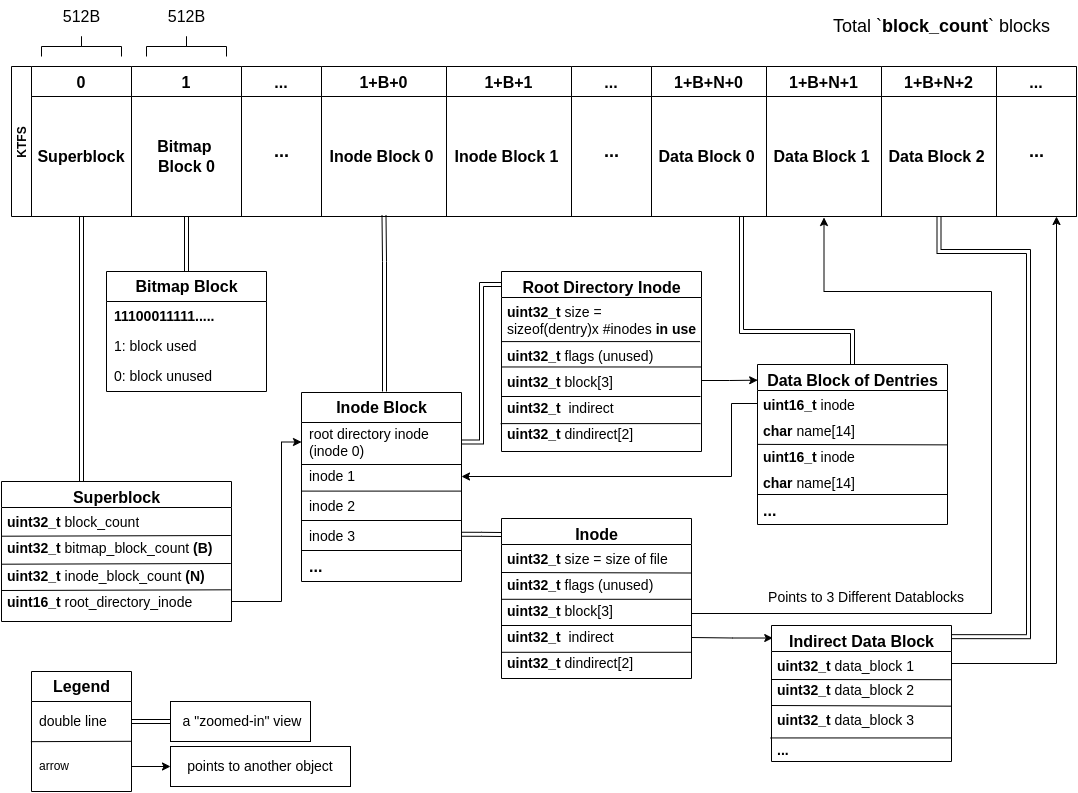
\includegraphics[scale=0.40]{ktfs.png}\\
	Layout of KTFS
\end{center}

KTFS is a block-based filesystem. We use a block size of 512B, which coincidentally matches with the block size of the VIRTIO device.
There are 4 types of blocks:
\begin{enumerate}
	\item Superblock (stores basic statistics of the file system image)
	\item Bitmap blocks (keeps track of which blocks are in-use)
	\item Inode blocks (stores index nodes (inodes), which contain info about each file)
	\item Data blocks (stores actual data)
\end{enumerate}

The first block is called the \textbf{superblock}. 
The superblock has four fields:
\begin{itemize}
	\item {\fix uint32\_t block\_count} - the total number of block in the file system
	\item {\fix uint32\_t bitmap\_block\_count} - the number of bitmap blocks
	\item {\fix uint32\_t inode\_block\_count} - the number of inode blocks
	\item {\fix uint16\_t root\_directory\_inode} - the index of the root directory inode (see below)
\end{itemize}
These fields only take up the first 14B of the 512B, so the remaining bytes are unused. The fields in the superblock are set
when creating the filesystem image (see \S \textbf{Building the File System}) and should not be modified by your OS.

The blocks following the superblock are the \textbf{bitmap blocks}.
The bitmap blocks contain "bits", as the name suggests.
Each bit indicates whether a block is used: 1 means used, 0 means free.
For example, the 0th bit of the 0th bitmap block corresponds to the 0th block of the filesystem.
If a block is free, then it can be used later when writing to a file or creating a new file.
When the filesystem image is created, the superblock, bitmap blocks, and inode blocks are all marked as in-use.
During filesytem image creation, the "disk size" is set and fixed, which means the number of bitmap blocks is also fixed.

The \textbf{inode blocks} contain the index nodes (inodes) of the files in the filesystem.
Each file is described by an inode that specifies the
file's size in bytes and the numbers of the data block (e.g. data blocks 1,5,10 ...) that make up the file.
During filesystem image creation, the number of inode blocks is set and cannot change.

Each inode only provide direct access to 3 data blocks through an array within the inode.
However, inodes additionally store 1 indirect data block number and 2 doubly-indirect data block numbers.
An indirect data block number points to a data block that contains an array of data block numbers, instead of actual data.
For example, if you want to access the 4th data block of a file, you will have to get the indirect data block number first 
(\eg {\fix inode.indirect = 11}),
get data block 11 from backing device, and read the first {\fix uint32\_t} (first 4B) of data block 11 (\eg 14).
Then, go to data block 14 and there will be actual data. The idea is the same for doubly-indirect blocks, except there's
one more layer of indirection: the doubly-indirect data block number points to a data block that stores an array of indirect data block numbers, 
which further points to indirect data blocks that store an array of "real" data block numbers.

Each indirect/doubly-indirect data block contains 512B (just like any other data block), but only the part of the indirect/doubly-indirect data block that points to data blocks necessary to contain the
specified size need be valid, so be careful not to read and make
use of block numbers that lie beyond those necessary to contain
the file data. The data blocks that make up a file are not necessarily contiguous
or in any specific order. You must use the data block numbers in the order specified in the inode and the indirect/doubly-indirect data blocks 
to access the correct data in the correct order.

There's one special inode called the root directory inode.
Instead of containing the actual data of a file in its specified data blocks, 
these data blocks contain the directory entries. KTFS does not support nested directories, so the root directory
is the only directory that you are required to support.
Each directory dentry (or dentries for short) contains an inode number and a string that contains the file name.
The size of each dentry is 16B: 2B for the inode number and 14B for the file name.
Note that because we need 1B for the null terminator, the maximum length of a file name is 13B (13 characters).
The "file size" specified in the root directory inode is equal to (the number of dentries) $\times$ (the size of each dentry). Therefore, you can
determine the number of files in the filesystem by checking the size field of the root directory inode. When you create or delete a file,
you must add/remove the dentry for that file and update the size appropriately.
For this file system, there is a 1:1:1 correspondence between files, dentries, and inodes. 
No two dentries should contain the same inode number or file name.

\textbf{Note:} Dentries \textbf{must} be contiguous to be able to use the file size properly. This is a strict requirement that 
filesystem images will follow and your filesystem driver must maintain. Keep in mind that ``contiguous'' here does not actually mean
contiguous in memory, just that if you were reading the root directory inode like a file, the first {\fix size} bytes would be the dentries.

In most cases, the \textbf{data blocks} can be seen as normal chunks of data in a file. That means when you open a file,
you should be reading data from and writing data to these actual data blocks. However, because of the root directory inode and indirect data blocks,
data blocks can contain different things. So, a data block can be classified into the following types depending on what data it contains:

\begin{enumerate}
	\item{"Real" data blocks (contains actual data of a file)}
	\item{Directory data blocks (pointed to by the root directory inode, contains directory entries)}
	\item{Indirect data blocks (contains an array of data block numbers)}
	\item{Doubly-indirect data blocks (contain an array of indirect data block numbers)}
\end{enumerate}

\textbf{Note:} Since the root directory inode is treated similar to a ``regular" inode, it can grow in size like other files with indirect and doubly-indirect data blocks. 
This means that the limiting factor on the number of files in a filesystem is typically the number of inodes.

\classsubsect{File Abstractions}

In order to make your filesystem driver, you should create a {\fix struct ktfs\_file}.
This will be the internal representation of a file that your filesystem driver uses
to keep track of the state of each file.
This structure should contain \emph{at least} the following fields (add more if you find it useful):

\begin{enumerate}

	\item{The {\fix io} struct associated with each file. The {\fix intf}
		field in this structure should be a pointer to an {\fix io\_intf} struct that
		contains the correct {\fix close, readat, writeat, cntl} function pointers to
		interface with the file.}


	\item{A \textbf{file size} member that stores the length of the file in bytes. This should
		be updated whenever write/writeat is called, if the length of the file has changed.}

	\item{The \textbf{directory entry} struct for this file. As a reminder, this contains the
		inode number for the file and the file name.}

	\item{A \textbf{flags} member for, among other things, marking this file
	      struct as ``in-use."}

\end{enumerate}

You need to have some way to keep track of the {\fix ktfs\_file} structs that correspond to currently 
opened files (array, linked list, etc.), so that future I/O operations can be performed on them.

\classsubsect{Building the File System}

The filesystem image needs to be made
in order for QEMU to read it and make it accessible to you (via VIRTIO). To do this,
we have provided you with 2 binary executables within the {\fix util/fs} directory.

\begin{itemize}
	\item {\fix mkfs\_ktfs} is a customized version of Linux {\fix mkfs} that generates a filesystem
	image according to the KTFS spec detailed above. This is how we will generate filesystem images to
	test and grade your filesystem driver.
	\item {\fix mkfs\_ktfs\_inorder} is a modified version of {\fix mkfs\_ktfs} that does not randomize the
	order of data blocks associated with each file. \textbf{This is provided for debugging purposes only} and
	will not be used to grade your filesystem driver. You must be able to interface with files that use non-contiguous data
	blocks.
\end{itemize}

We have also provided you with a 3rd binary executable, {\fix unmkfs\_ktfs}. This program ``unwraps" the
files contained with a KTFS filesystem image to allow you to parse them on your own. You may find this useful when
implementing the write/writeat functions in your filesystem driver, since these functions will modify your actual
filesystem image and persist between QEMU shutdowns.

{\fix mkfs\_ktfs} usage is as follows:
\begin{verbatim}
./mkfs_ktfs [filesystem_image] 
            [disk_size in K, M, or G] 
            [inode_count] 
            [file1] [file2] ...
\end{verbatim}
In order for your filesystem image to work with our existing {\fix Makefile}, you should name
the image {\fix ktfs.raw} and put it in the {\fix sys} directory. 

An example:
\begin{verbatim}
	./mkfs_ktfs ../../sys/ktfs.raw 8M 16 ../../usr/bin/hello ../../usr/bin/trek
\end{verbatim}

This would create a {\fix ktfs.raw} file in the {\fix sys} directory with a total size of 8MiB and 16 inodes (\ie, 1 inode block).
{\fix hello} and {\fix trek} would be the only 2 files in the filesystem image, with the rest of the inodes free.

Since we cannot have fractional data blocks, your disk size should always be a multiple of 512 (KTFS block size).
The number of inode blocks is also rounded up, since we cannot have fractional inode blocks. When interfacing with the filesystem, you can
consider any block marked as an "inode block" as able to be used to store inodes. In other words, the total number of possible inodes in your
file system will always be a multiple of 16.
However, bitmap blocks may be "partially" used. Be careful to not read/write past the size of the filesystem image.

\textbf{Note:} Make sure you are running your {\fix mkfs\_ktfs} binary and not the Linux {\fix mkfs} function.

The files in your filesystem image are also given as arguments to {\fix mkfs\_ktfs}. You can (and
should) provide multiple files in order to create a full filesystem image. All the metadata related 
to these files will be prepared for you, including the superblock and other structures that you've
read about in \textbf{Appendix A} already. All of these blocks will be put in order according to the 
spec above and stored in your filesystem image (\ie, {\fix ktfs.raw}). This means that the filesystem 
image is already compliant with the KTFS spec.

To load a user program into the filesystem image, you need to compile it to an executable
binary. This can be done by using the {\fix Makefile} in {\fix usr}. If you want to change
a file in the filesystem or add/remove files (without using your filesystem driver), 
you \textbf{must} remake the filesystem image each time.

\classsubsect{The Blob}
The blob will be created as an object file and is not part of the regular filesystem. 
It is a tool for debugging and testing. If {\fix blob.raw} exists in your {\fix sys} directory,
the {\fix Makefile} 
will input the file contents of {\fix blob.raw} to a read-only data section starting from 
{\fix \_kimg\_blob\_start} to {\fix \_kimg\_blob\_end}. These addresses can be obtained via {\fix extern}. 
If you want to use the blob, simply rename the relevant file to {\fix blob.raw} in the {\fix sys} 
directory and add the object file when you build your kernel image ELF file as well as {\fix extern} both 
addresses in your code to access the blob.
\vfill



\else
% Do nothing
\fi

\ifnum\renderappB = 1

\pagebreak
\classsect{Appendix B: I/O Devices}

\classsubsect{Overview}

For Checkpoint 1, you must support a variety of devices, most of which use the {\fix io} abstraction. When interacting with devices, abstraction is necessary. Historically, companies have come together in consortiums related to networking and inter-device communication (see PCI-E, USB, CCIX). These interconnects enable fast, standardized communication between devices.

QEMU is simulating devices and their interconnects. Your filesystem image, for example, (see \textbf{Appendix A}) will be managed by the QEMU block device.

\classsubsect{I/O Operations}

The kernel will interact with devices using the struct {\fix io}. Each struct {\fix io} 
contains a pointer to a struct {\fix iointf}, which in turn contains pointers to {\fix close}, 
{\fix ctntl}, {\fix read}, {\fix write}, {\fix readat}, and {\fix writeat} functions specific to each device driver. 
Note that not all these functions need to be implemented - if the device driver does not implement the function, the pointer
can be NULL. Under the hood, these callback functions to the device drivers will use the memory-mapped 
I/O regions to communicate with devices.

\classsubsect{I/O Diagram}

\hspace{-1.7cm}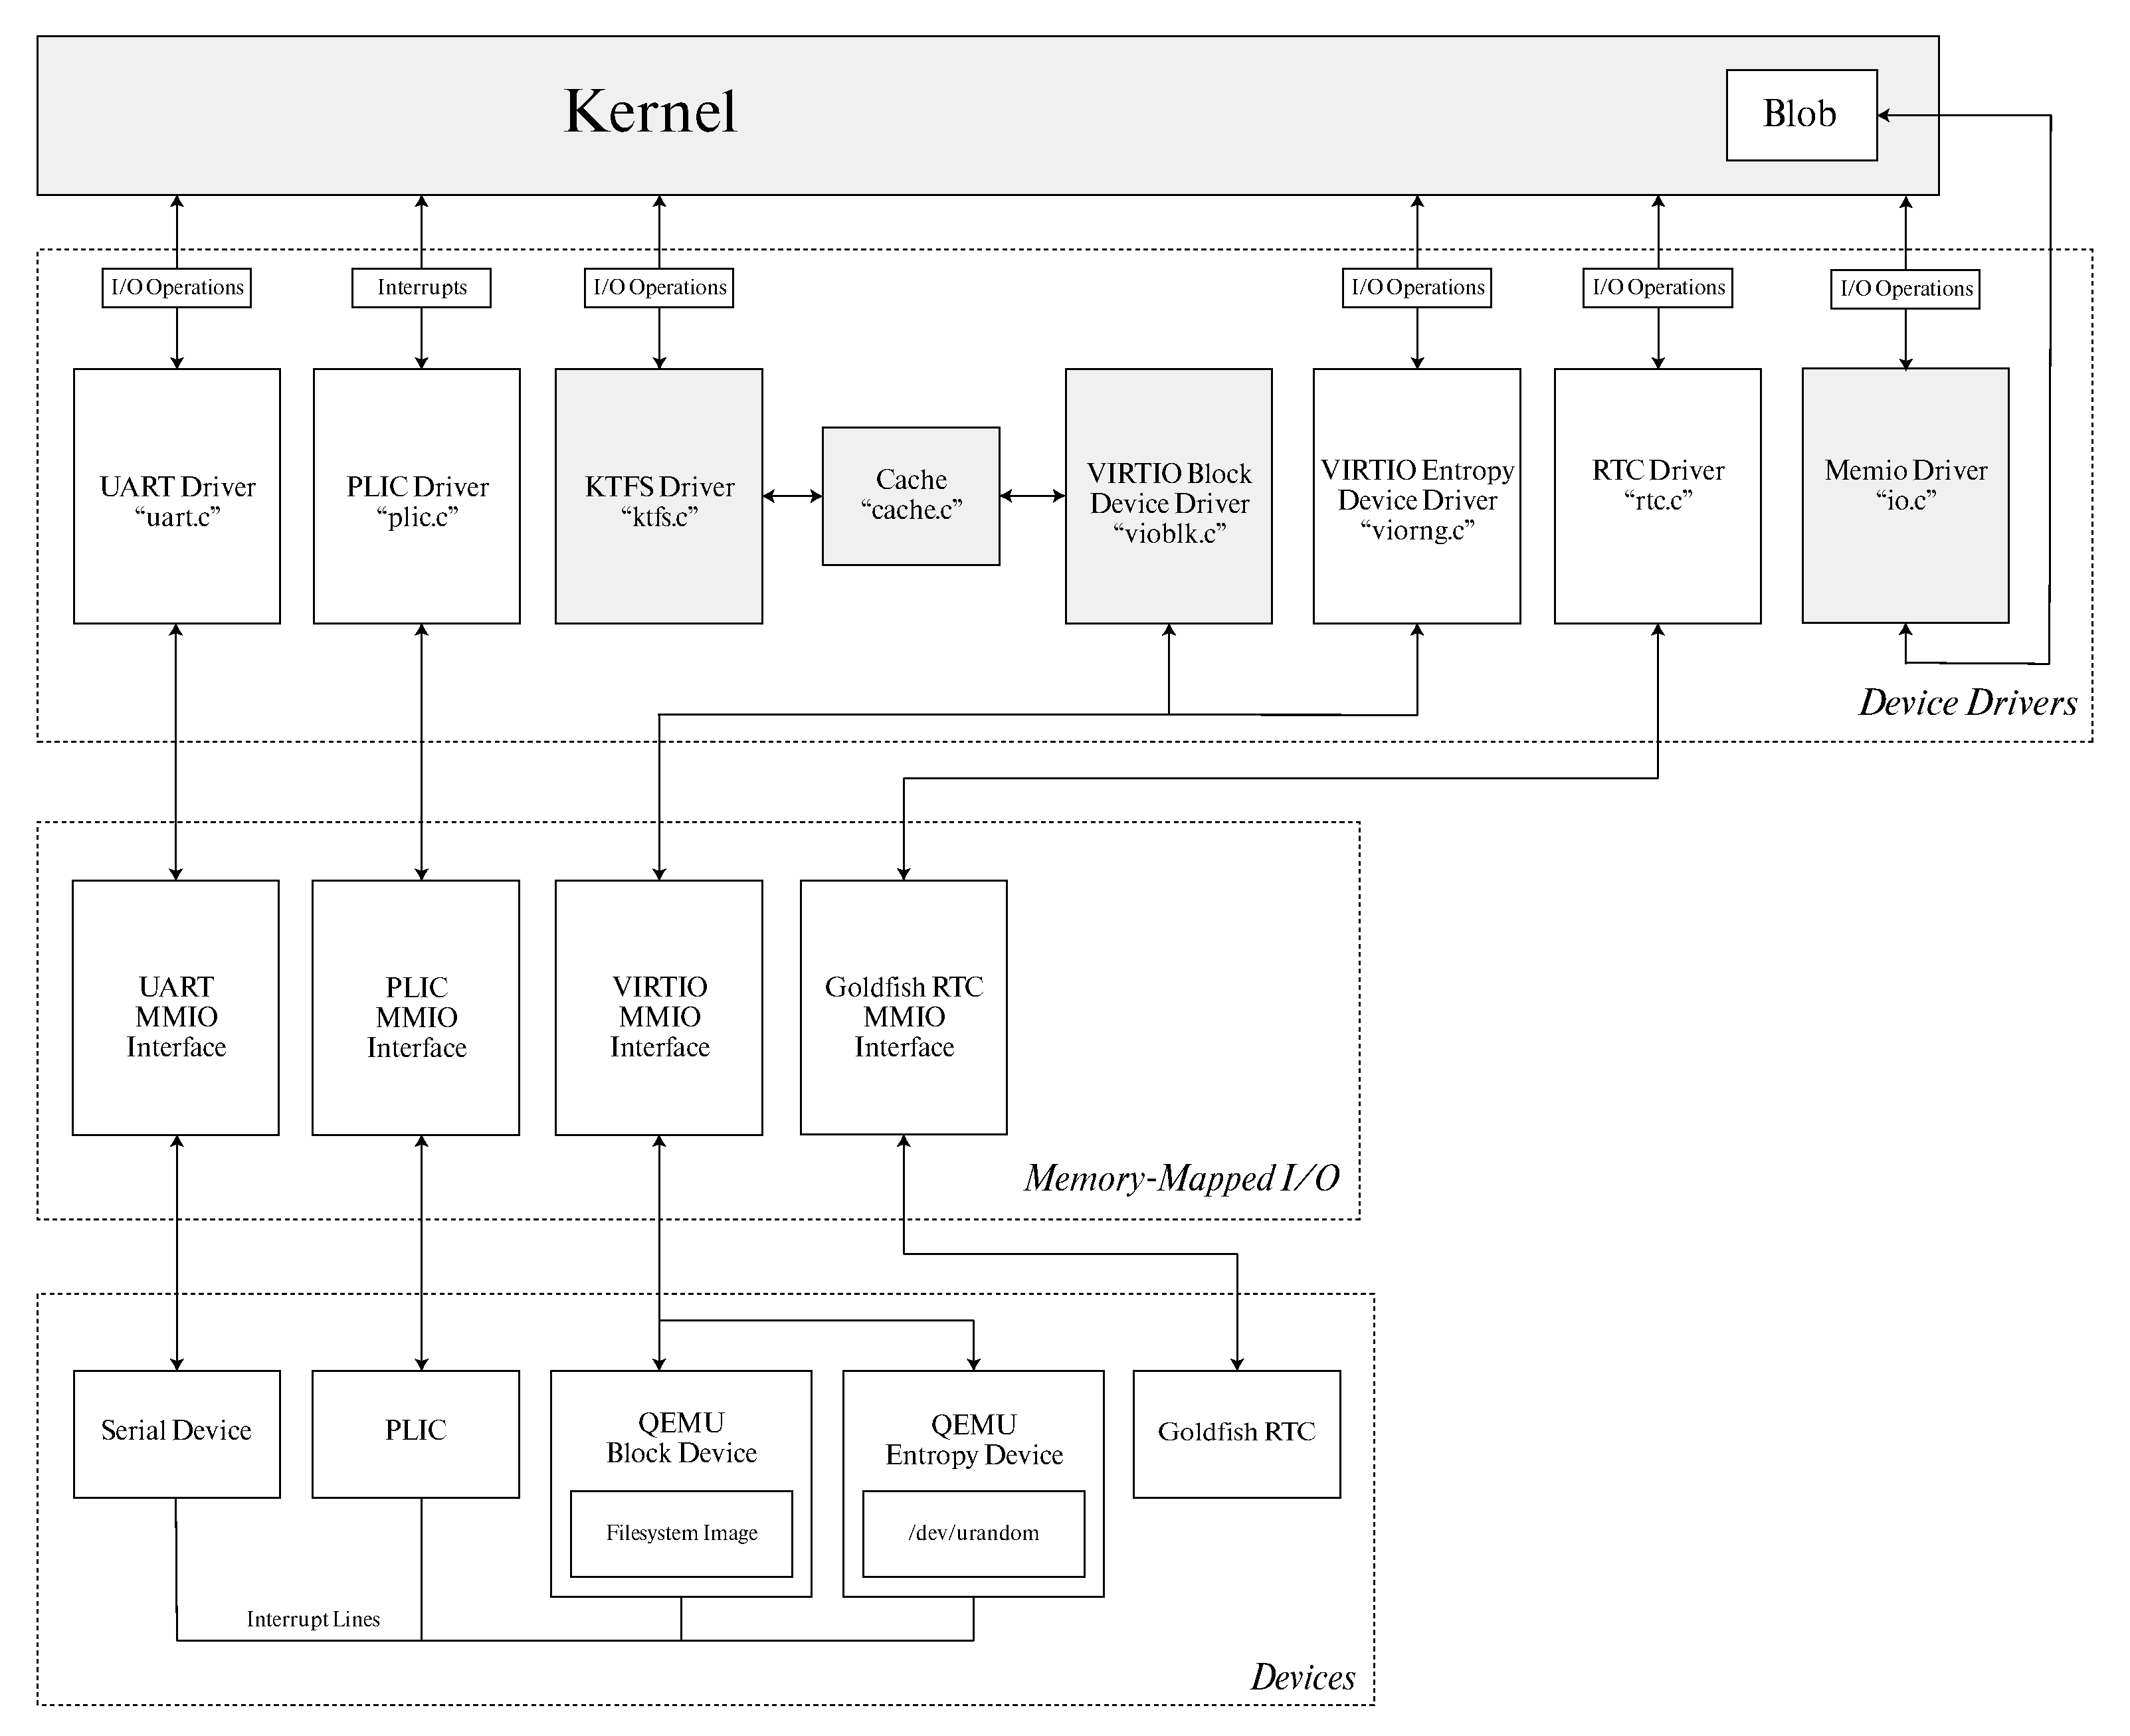
\includegraphics[scale=0.35]{io.pdf}\\
\begin{center}
    The shaded blocks are the parts that you will write as part of MP3.
\end{center}
% \begin{center}
%     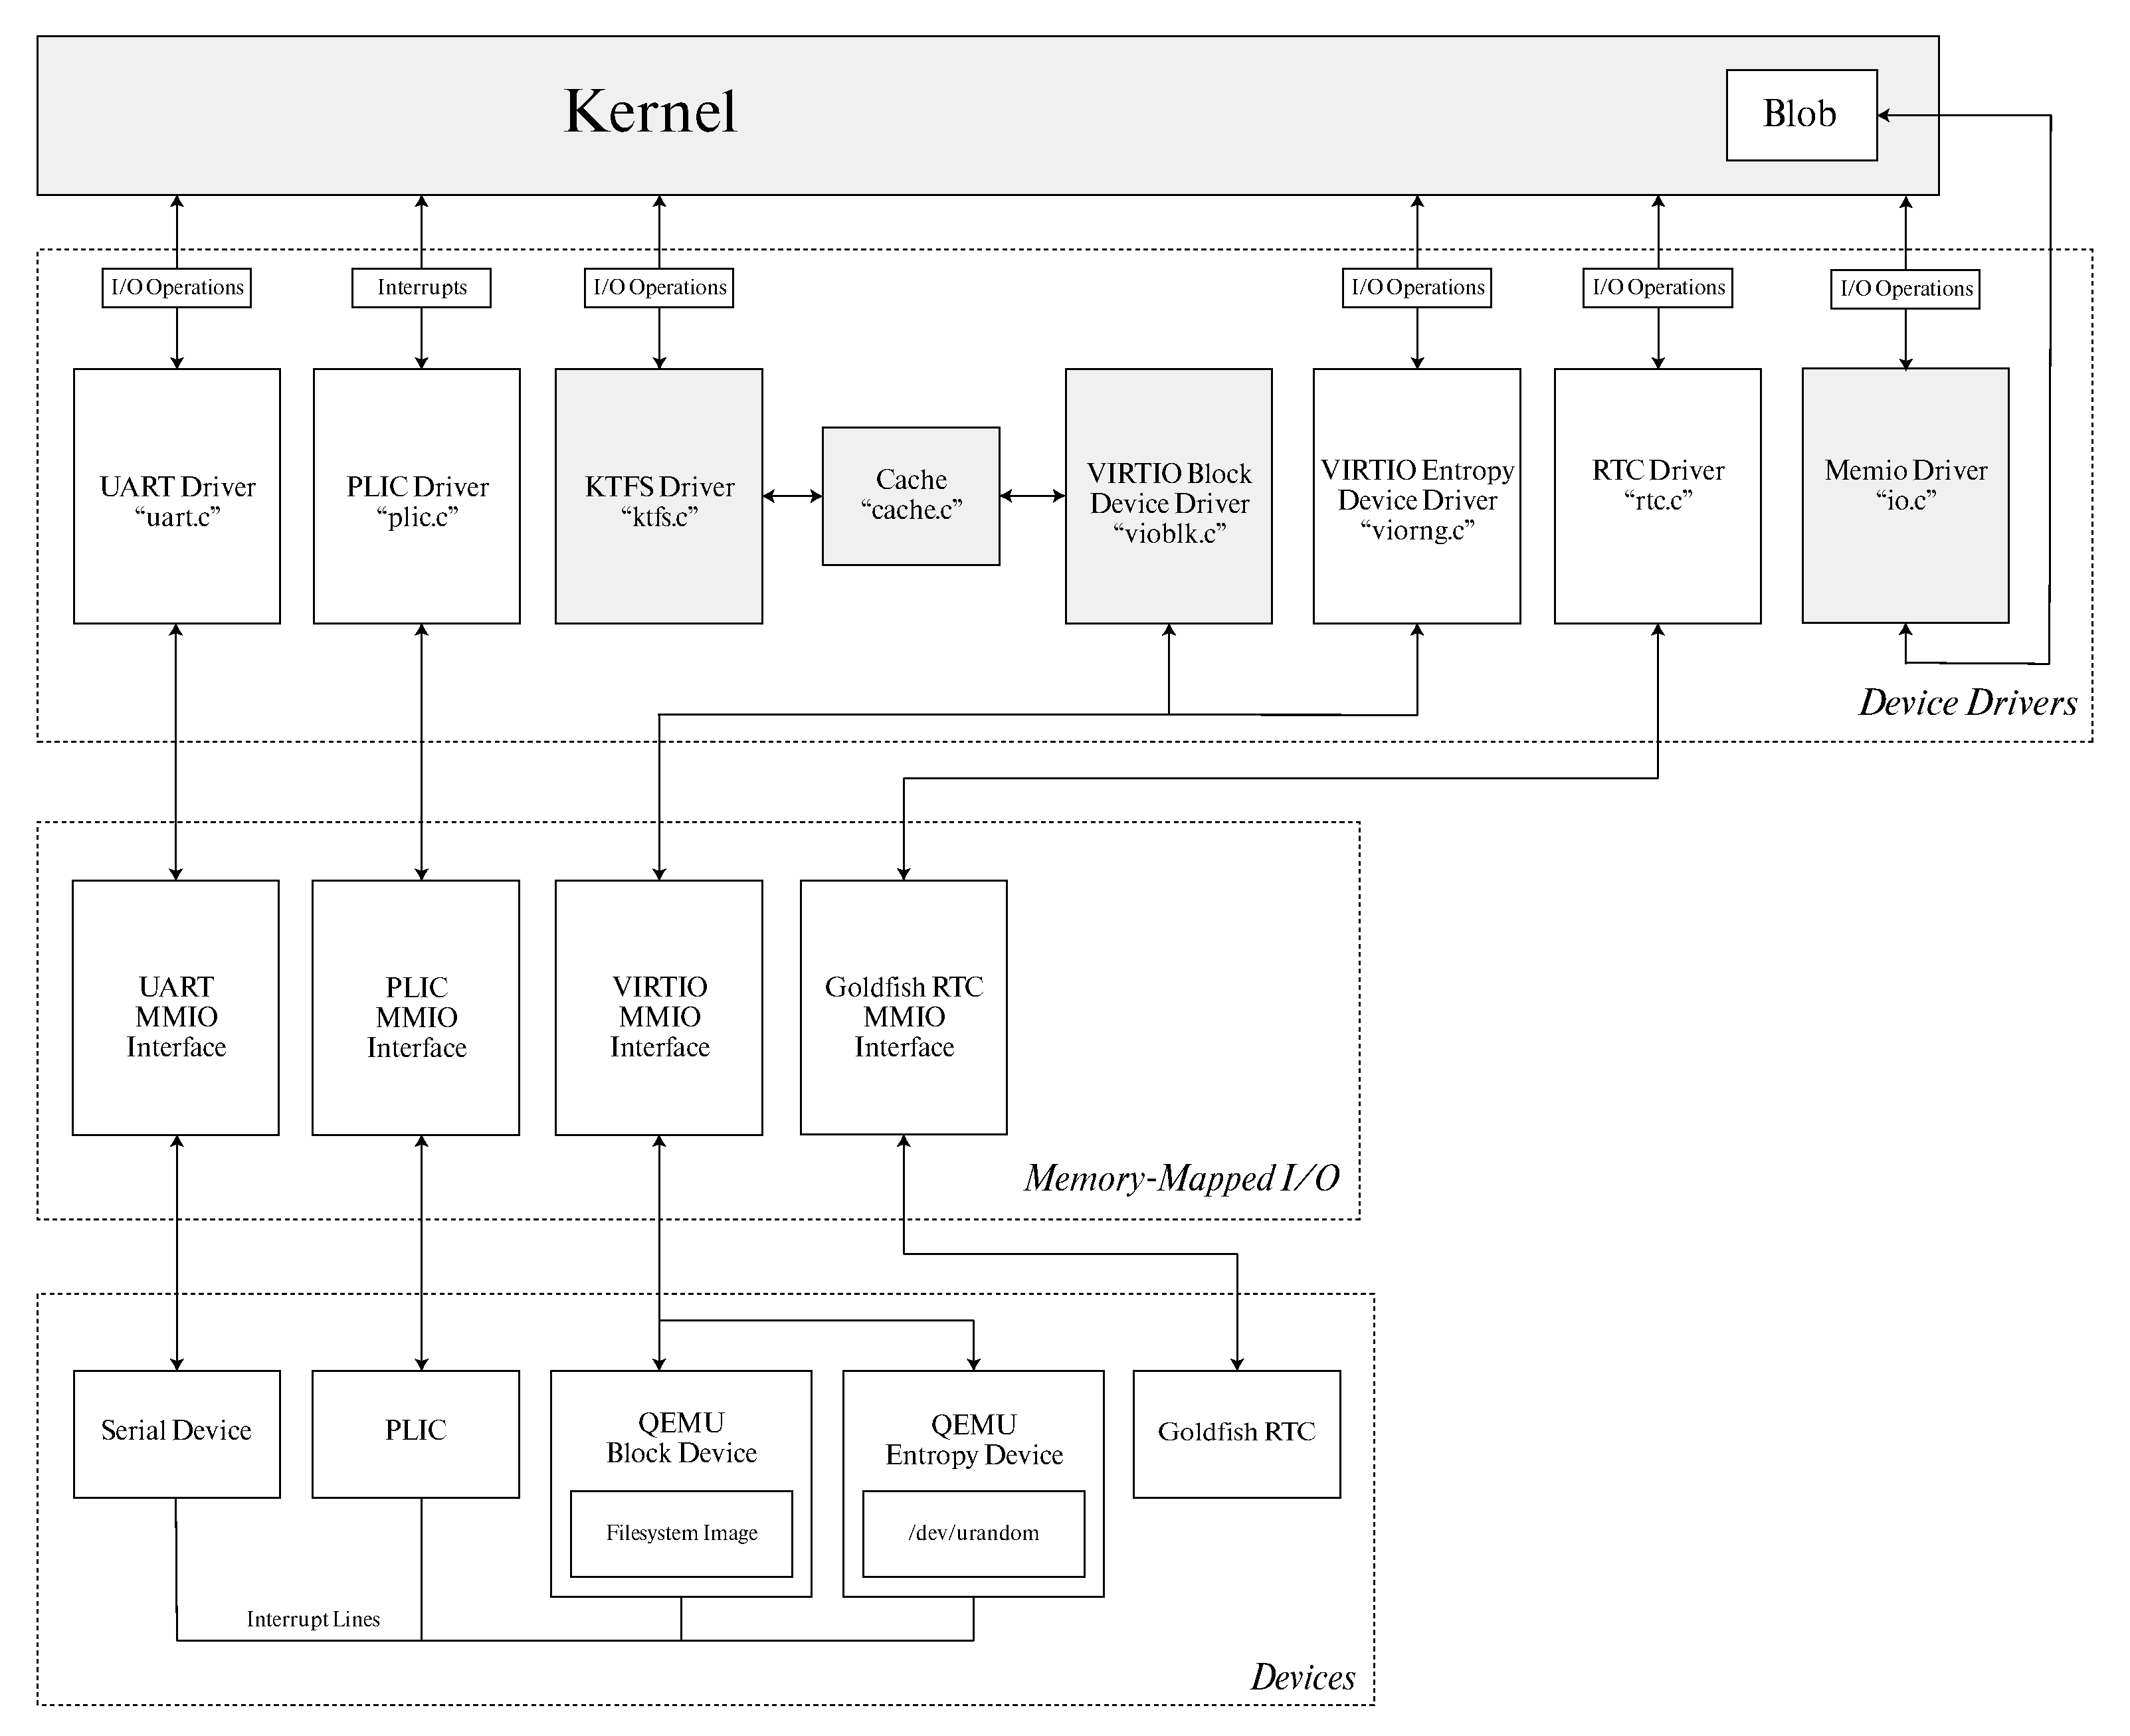
\includegraphics[scale=0.45]{io.png}\\
%     The shaded blocks are the parts that you will definitely modify as part of MP3.
% \end{center}
\vfill

\else
% Do nothing
\fi

\ifnum\renderappC = 1

\classsect{Appendix C: The Process Abstraction}
	
	\classsubsect{History}
	
	The process abstraction in Unix like systems is a critical part of understanding an operating system's inner workings.
	Historically, processes were the first abstraction over a user program rather than threads. User programs were seen as
	having a single flow of instruction and resided in separate memory spaces. As computer hardware advanced and provided stronger
	computing, it became desirable to have multiple streams of instructions (threads) running within a single address space. 
    For Checkpoint 2 we will only consider processes that contain only a single thread.
	
	\classsubsect{Overview}
	
	The Linux kernel's smallest abstraction over a stream of instructions is a thread. For a UNIX-like system (like ours), 
	each process by default will be spawned	around a main thread. This main thread is what is scheduled by the operating system.
	
	A process being scheduled by the kernel to run is just the process's thread being put on the ready list and a process running
	is just the thread associated with the process running (as the current thread).
	
	On top of owning a thread, each process also owns a virtual memory space. This virtual memory space is represented by a 3-level page table. You can read more about the paging and virtual memory
	in \textbf{Appendix D}.
	
	In addition, a process should also keep track of files and devices that it's interacting with. 
	Note that we have a common interface for files and devices (\texttt{io})
	
    The process abstraction provides 3 key guarantees to a user process:

    \begin{itemize}
        \item \textbf{Protection:} Assures that a malicious process cannot corrupt, fault or deny other user processes.
        \item \textbf{Virtualization:} Creates the illusion to a process that resources are boundless and only used by that process, \ie virtual memory, illusion of concurrency with scheduling, etc.
        \item \textbf{Abstraction:} Abstracts away implementation details and provides a common interface
    to user processes, \eg a user program opening a file is the same code regardless of the file
    system being backed by an memio or a vioblk device. They are covered by the same system call.
    \end{itemize}
    
    \classsubsect{Context Switching between User-Mode and Supervisor-Mode}
    
    Context switching between two privilege levels fundamentally requires two instructions with two unique properties:
    
    \begin{enumerate}
        \item An instruction to go from a lower privilege level to a higher privilege level
        \item An instruction to go from a higher privilege level to a lower privilege level
    \end{enumerate}
    
    \textbf{The ECALL Instruction:}

    The environment call ({\fix ecall}) instruction will be our way of going from a lower 
    privilege level (user-mode) to a higher privilege level (supervisor-mode). It is meant to be used by user-mode software
    to make a service request to a higher privilege context.
    
    Reading the description for the {\fix ecall} instruction in the RISCV Privileged ISA manual we can see that it will trigger an exception 
    which should be delegated to the supervisor-mode trap handler. This exception being triggered from user-mode will have the following effects:
        \begin{enumerate}
            \item The {\fix sepc} register is loaded with the virtual address of the instruction that triggered the exception (\ie the {\fix ecall} instruction itself).
            \item The {\fix scause} register contains the cause code for the exception (the cause code for an environment call from user-mode).
            \item The {\fix sstatus} register's Supervisor Previous Privilege bits (SPP) will be set to 0 to indicate that it is a trap from user-mode.
            \item The {\fix sstatus} register's Supervisor Previous Interrupt Enable bits (SPIE) will indicate whether or not supervisor-mode interrupts
            were enabled prior to trapping into supervisor-mode. 
            \item The {\fix sstatus} register's Supervisor Interrupt Enable bits (SIE) will be cleared to disable supervisor-mode interrupts while in
            supervisor-mode.
        \end{enumerate}
    
        
     \textbf{The SRET Instruction:}

     The supervisor return ({\fix sret}) instruction is what we'll use to transition from a higher-privilege level (supervisor-mode) to a lower
     privilege level (user-mode). It is meant to return to user-mode once a user request has been completed.
     
     Reading the description for the {\fix sret} instruction in the RISCV Privileged ISA manual we can see that an {\fix sret} in supervisor-mode will 
     return to a lower privileged mode (user-mode) with the following effects:
        \begin{enumerate}
            \item The {\fix sstatus} register's SIE bit will be set to SPIE.
            \item The {\fix sstatus} register's SPIE bit will be set to 1.
            \item The {\fix sstatus} register's SPP bits will determine the execution privilege mode after {\fix sret}.
            \item The {\fix sstatus} register's SPP bits will be set to the least-privileged supported mode (user-mode).
            \item The {\fix pc} register is set with the value of {\fix sepc}.
        \end{enumerate}
     
     Now that we know the effects of {\fix ecall} and {\fix sret}, we can reason about how to use these
     instructions during context switches. There are two specific cases to consider:
     
     \begin{itemize}
         \item \textbf{Switching to supervisor-mode from user-mode:} This type of switch is the most
         straightforward transition and does not require any preparation. You can just use the
         {\fix ecall} instruction.
         \item \textbf{Switching to user-mode from supervisor-mode:} Since our kernel initially boots into supervisor-mode,
         it can be a bit tricky to figure out how to use {\fix sret} to transition into user-mode. This confusion
         may come up because at first glance {\fix sret} requires a prior user program to have trapped into 
         supervisor-mode (so that the SPP and SPIE bits will be pre-populated with values). However, if this is the 
         first time a user program is being executed there can't be any prior user-mode trap frame and SPP and SPIE cannot
         be filled in. It is up to the process\_exec function to fill in the proper values for SPP and SPIE so that
         {\fix sret} can properly jump to a user-space function.
     \end{itemize}
    
\else
% Do nothing
\fi

\ifnum\renderappD = 1
\classsect{Appendix D: RISC-V Paging}

\classsubsect{Illinix Mappings}

\begin{center}
	\includegraphics*[scale=0.5]{kernel_memlayout.png}
\end{center}

\pagebreak
\classsubsect{Sv39}

RISC-V offers a few different paging schemes, each of which offers a different virtual memory size.
We are using Sv39 for this MP. Each {\fix struct pte\_t} (defined in {\fix memory.c}) describes a
page table entry specific to Sv39. You will need to look at the RISC-V privileged docs to 
learn more about each field: \href{https://riscv.org/wp-content/uploads/2017/05/riscv-privileged-v1.10.pdf}{here}.

Virtual memory address translation, also called {\fix paging}, is a hardware-level tool that supports process virtualization.
When paging is enabled and the machine is in umode, the hardware will translate all user-program memory accesses from virtual to physical
addresses.

Multiple programs may be staged to execute at the same address. Memory virtualization allows each process to
execute with the idea that they have the entire memory space at their disposal, and ensures that the operating
system can manage many programs executing in parallel.

To use the QEMU console (useful in debugging) you can add the following line in {\fix src/kern/Makefile}
where you set your {\fix QEMUOPTS}

\begin{center} 
	{{\fix QEMUOPTS += -monitor pty}}
\end{center}

When running {\fix make run-kernel}, your will see another {\fix /dev/pts/N} that you will need to connect to
in order to interact with your QEMU console. To view the virtual memory mappings of your system, you can run {\fix info mem} in your qemu console.
\vfill

\pagebreak

\else
% Do nothing
\fi

\ifnum\renderappE = 1
\classsect{Appendix E: Makefiles}

For MP3, you should learn how to read and modify your {\fix Makefile}. You have already done this occassionally 
for MP1 and MP2, so we expect that you are familar with the basic layout.

\vfill
\pagebreak
\else
% Do nothing
\fi

\ifnum\renderappF = 1

\classsect{Appendix F: Symbolic Links}

This is a mini-tutorial on how to use {\fix ln} in UNIX. If you want more information, try {\fix man ln}.

Create a symbolic link to a file or directory:

{\fix ln -s /path/to/file\_or\_directory path/to/symlink}

Overwrite an existing symbolic link to point to a different file:

{\fix ln -sf /path/to/new\_file path/to/symlink}

\else
% Do nothing
\fi

\ifnum\renderappG = 1

\classsect{Appendix G: Signals}

For extra credit,
your OS can provide an infrastructure for user-level signals, similar to
Linux.  The table details the signals that will be supported.

\vspace{6pt}
\centerline{
	\begin{tabular}{|c|c|c|}
		\hline
		\textbf{Signal name} & \textbf{Signal number} & \textbf{Default action} \\
		\hline
		{\fix DIV\_ZERO}     & 0                      & Kill the task           \\
		{\fix SEGFAULT}      & 1                      & Kill the task           \\
		{\fix INTERRUPT}     & 2                      & Kill the task           \\
		{\fix ALARM}         & 3                      & Ignore                  \\
		{\fix USER1}         & 4                      & Ignore                  \\
		\hline
	\end{tabular}
}
\vspace{6pt}

The {\fix set\_handler} system call changes the default action taken when a
signal is received: the {\fix signum} parameter specifies which signal's
handler to change, and the {\fix handler\_address} points to a user-level
function to be run when that signal is received.  It returns~0 if the handler
was successful set, and~-1 on failure.  If {\fix handler\_address} is NULL
(zero), the kernel should reset the action taken to be the default action.

	{\fix DIV\_ZERO} should be sent to a task when the x86 processor generates a
divide-by-zero exception while executing user-level code.  {\fix SEGFAULT}
should be sent when any other exception occurs, including any illegal
instructions, illegal memory references, page faults, general protection
faults, illegal opcodes, \etc~~The {\fix INTERRUPT} signal should be sent when
a CTRL+C is pressed on the keyboard.  The {\fix ALARM} signal should be sent
to the currently-executing task (there is only one currently-executing task in
this OS) every 10 seconds.  This should be implemented by knowing at what rate
the RTC's Periodic Interrupts occur, counting how many Periodic
Interrupts have occurred, and sending an {\fix ALARM} signal after 10 seconds
have elapsed.  Finally, {\fix USER1} is user-defined and can be used to
implement any other signal of your choosing.

Signals should only be delivered to a task when returning to user space from
the kernel, so you'll want to add some code in your return-to-user space
linkage to check for pending signals.  To support signal delivery, you should
use a mechanism similar to what Linux uses:

\begin{enumerate}

	\item

	      Mask all other signals.

	\item

	      Set up the signal handler's stack frame.  You'll need the current value of the
	      user-level ESP register to find the user's current stack location.  The signal
	      handler stack frame goes directly above this on the stack.

	      The signal handler stack frame is shown in Figure \ref{fig:signal-stack}.
	      Setting up the signal handler stack frame involves: copying a return address
	      and a signal number parameter to the user-level stack, copying the process's
	      hardware context (see Figure \ref{fig:hwcontext}) from the point when the
	      program was interrupted for the signal, and copying a small amount of assembly
	      linkage to the user-level stack that calls {\fix sigreturn} when the signal
	      handler is finished.

	\item

	      Finally, execute (in user space) the handler specified in the signal
	      descriptor.  No other information needs to be passed to the signal handler (no
		      {\fix siginfo\_t} structure like the modern Linux signals).

\end{enumerate}

When the user-level signal handler returns, it will use the return
address you have copied on its stack, which will jump to the assembly linkage
(also on the stack).  This assembly linkage should make the {\fix sigreturn}
system call (using the standard {\fix int \$0x80} user-level system call
calling convention).

The {\fix sigreturn} system call should copy the hardware context that was on
the user-level stack back onto the processor.  To find the hardware context,
you will need to know the user-level value of ESP (will be saved by your
system call handler) as well as the exact setup of the user-level stack frame.
To copy the hardware context back onto the processor, you will actually
overwrite the kernel's copy of the process's hardware context that was saved
on the \textit{kernel} stack when it handled the {\fix sigreturn} system call.
In this way, when the {\fix sigreturn} system call handler returns to
user space, the hardware context will automatically be copied back onto the
processor by your return-from-kernel code that you have already written.  One
thing to be careful of: you'll probably have system calls set up to return a
value (in EAX) to user space.  Be sure you don't clobber the user's EAX value
from its hardware context with a bogus ``return value'' from {\fix sigreturn}
-- have {\fix sigreturn} return the hardware context's EAX value so that you
won't have to special-case the return from {\fix sigreturn}.

\begin{figure}
	\begin{minipage}[b]{.5\linewidth}
		\centering
		\includegraphics[height=1.5in]{notes-signals-frame.eps}
		\vspace{1in}
		\caption{User-level signal handler stack frame.}
		\label{fig:signal-stack}
	\end{minipage}
	\begin{minipage}[b]{.5\linewidth}
		\includegraphics[width=3in]{ptregs-modified.eps}
		\caption{Hardware context structure.}
		\label{fig:hwcontext}
	\end{minipage}
\end{figure}

Shown in Figure~\ref{fig:hwcontext} is a slightly-modified version of the
	{\fix struct ptregs} structure that Linux uses for its hardware context; this
modified structure is what you should use in this MP.  The ``Error Code /
Dummy" field has been added to the hardware context to simplify exception
handling.  For some exceptions, the processor pushes an error code onto the
stack after XCS (for example, page faults do) whereas other exceptions do not
(divide-by-zeros do not).  For exceptions that do not push this error code,
your exception handler should push a dummy value to take up the error code
slot\footnote{Linux's \texttt{struct ptregs} does not include this error code
	field; instead, the Linux exception handlers play tricks with the stack and
	registers to avoid adding an extra slot.}.  x86 interrupts never push the
error code, so you must also push a dummy value in all of your interrupt
handlers and the system call handler.  You can find documentation about which
exceptions push error codes (and much more about exceptions) in \textit{Volume
	III: System Programming} of the Intel ISA manual on the Tools, References, and
Links section of the website.

Finally, signal handling information should go in the process control block (PCB).
You will need to keep track of pending signals, masked signals, and handler
actions / addresses for each signal.  Much information on Linux's
implementation of signals (which your implementation will closely match) can
be found in \textit{Understanding the Linux Kernel} chapter 10.\\

\vfill
\pagebreak

\else
% Do nothing
\fi

\ifnum\renderappH = 1
\pagebreak

\classsect{Appendix H: Troubleshooting}

	\classsubsect{Debugging with gdb}

	\emph{``If debugging is the process of removing bugs, then programming must be the process of putting them in.'' -Edsger W. Djikstra}

	One of the most important skills you can have as a software engineer is being able to debug.
	While print statements are useful and easy to implement, using a real debugger like gdb will
	allow you to find and solve your problems much more quickly. If you invest time into learning
	it at the start of this MP, it will pay dividends for the rest of the assignment and future classes.
	Many ECE 391 alumni (including course staff) have said that the most important thing they learned from the course
	was not how to make an operating system, but how to debug effecitvely on their own. While course
	staff are there to help you, they are not there to handhold you and it is expected that you are able
	to debug on your own, especially with gdb.

	\subsubsection{Debugging the Kernel}

	This section describes how to set up your kernel to work with gdb. This will 
	allow you to step through kernel and user program code if it is compiled 
	with debugging symbols ({\fix -g}).

	Whenever a change is made to your kernel, you should rebuild your kernel
	using {\fix make}. For the purposes of this appendix, we'll be describing debugging with
	the {\fix kernel.elf} kernel image, which we've given you. If you're using a different
	kernel image, use that instead. You can create 
	different kernel images by writing an appropriate {\fix main\_<prog>.c} file
	and adding it to the {\fix Makefile}.

	To launch QEMU and have it wait for remote debugging, you must include the
	{\fix -S} flag, which we have done for the command {\fix make debug}. This
	will launch your {\fix kernel.elf} kernel image as normal, but no instructions
	will execute until you connect to it with gdb and run {\fix continue}.

	Once you've launched your kernel, you need to open a second terminal and run
	
	{\fix riscv64-unknown-elf-gdb [kernel image]}

	This will run the correct version of gdb and load the debugging symbols from
	your kernel image, allowing you to set breakpoints and step through the code.
	We have included a {\fix .gdbinit} file in the {\fix sys} directory, which
	executes a few commands on gdb startup --- this should cause it to automatically 
	connect to your QEMU instance. To use the {\fix .gdbinit} file, simply launch
	gdb from the {\fix sys} directory.\\

	\textbf{Note:} The first time you use a {\fix .gdbinit} file, you might get a message
	that looks like this

	{\fix warning: File "/path/to/src/kern/.gdbinit"
	auto-loading has been declined by\\
	your `auto-load safe-path'.\\
	To enable execution of this file add\\
	add-auto-load-safe-path /path/to/src/kern/.gdbinit\\
	line to your configuration file "\raisebox{0.5ex}{\texttildelow}/.config/gdb/gdbinit".}

	In order to resolve this, you should simply follow the instructions that gdb gives you
	and add the path. You may have to use {\fix mkdir} to make
	the {\fix \raisebox{0.5ex}{\texttildelow}/.config/gdb} directory before using your favorite
	text editor to add the {\fix add-auto-load-safe-path /path/to/src/kern/.gdbinit} line into
	{\fix \raisebox{0.5ex}{\texttildelow}/.config/gdb/gdbinit}. You only need to perform this setup
	process once per {\fix .gdbinit} file, even if you modify it in the future. It is \textbf{highly recommended}
	that you use the {\fix .gdbinit} file to save you the trouble of having to connect to the QEMU instance every time.
	
	\textbf{Note:} You may need to modify the
	{\fix target remote 127.0.0.1:1234} line in your {\fix .gdbinit} file to match
	the port your QEMU instance uses. The {\fix -s} flag provided to QEMU allows it to use
	the default port (1234), but if you are having trouble connecting with that port, you can 
	explicitly specify which port to use in the QEMU command. Then, modify your {\fix .gdbinit} file
	to match.

	\subsubsection{Debugging User Programs}

	If you want to set breakpoints or step through a user program, things are
	slightly more complicated. Since {\fix kernel.elf} (or whatever your kernel
	image is) does not contain the user program, we need to add the debugging
	symbols for it separately into gdb.

	First, you need to compile your user program with debugging symbols enabled.
	In the {\fix Makefile} we have provided, we have already enabled debugging symbols
	({\fix -ggdb3}). If you write your own user program, you can
	add it to the {\fix Makefile}. To find the address of the program itself, run

	{\fix readelf -Wl [program binary]}

	This gives you information on where different sections of your program are loaded.
	Find the executable section ({\fix E} flag) and note down the {\fix VirtAddr}.
	For checkpoint 1, it should be located around {\fix 0x80100000}. For later checkpoints, 
	once you have virtual memory enabled, it should be located between {\fix USER\_START\_VMA} 
	and {\fix USER\_END\_VMA}. If using {\fix UMODE} and virtual memory, be sure to enable the {\fix UMODE}
	flag within {\fix usr/Makefile}.
	You will need to manually tell gdb that this is where the program starts.

	To do this, open gdb as normal with {\fix make debug}, then use the {\fix add-symbol-file}
	command to add your user program. An example would be

	{\fix add-symbol-file ../user/bin/hello 0x0000000080100000}

	If there is a prompt, hit "Y" to accept. Now, you should be able to set breakpoints
	and step through the user program. You will need to run this command every time that
	you re-open gdb --- if you find yourself using it constantly, consider adding it to
	your {\fix .gdbinit}.

	\subsubsection{Useful gdb Commands}

	The best way to get good at using gdb is to actually use it. To get you started, here are some
	pages with gdb commands we found useful. There are a lot more out there, and it is highly encouraged
	that you spend time looking at the gdb man page ({\fix man gdb}) and any other online resources for gdb.

	\textbf{Note:} Your code may run noticably slower when using gdb, especially if you are performing a lot of comparisons.

	\begin{itemize}
		\item \href{https://ccrma.stanford.edu/~jos/stkintro/Useful_commands_gdb.html}{Stanford CCRMA gdb Guide}
		\item \href{https://sourceware.org/gdb/current/onlinedocs/gdb.html/index.html}{gdb Wiki}
	\end{itemize} % add any other useful gdb pages here

	Here are some additional useful gdb tips and tricks:

	\begin{enumerate}
		\item Manipulating Local Variables

		You can use arithmetic operations (+, -, *, /, etc.) as well as pointer arithmetic (*, \&, [], etc.)
		on variables in gdb. You can also cast variables or numbers, just like in C. To access the fields of a struct,
		use {\fix .} or {\fix ->} appropriately. This is most useful with {\fix p[rint]}.

		\item Watchpoints

		You can use watchpoints to "watch" the value of a variable and trigger a breakpoint if it changes. Use
		{\fix watch <var>} to set a watchpoint on a variable.

		\item Conditional Breakpoints and Watchpoints
		
		You can use the format {\fix break WHERE if CONDITION} to set a conditional breakpoint, where
		it will only happen if a certain condition is met. For example, {\fix watch i if i == 100} would
		break if {\fix i == 100}. If your variable is constantly being modified, this can cause a major slowdown
		in your program execution.

		\item Printing Registers

		Using {\fix i[nfo] r[registers]} can be useful to see all (or any specific) registers, but all registers can also
		be referenced with the {\fix \$<register name>} variable. For example, {\fix p/x \$sp} prints out the value of {\fix sp}
		in hexadecimal. However, for CSRs, it is recommended you use {\fix i[nfo] r[egisters]} in order to get "pretty printing".

		\item gdb History

		By adding {\fix set history save on} to your {\fix .gdbinit} file, you can access the history of commands from previous gdb
		sessions. You can also further customize the file location and history depth.

		\item {\fix until} and {\fix finish}

		When using gdb, stepping through long for loops can be somewhat annoying. Typically, you will set a breakpoint after the loop
		and use {\fix c[ontinue]} to skip over it. However, you can also use the {\fix until <line number>} command to skip without having
		to set a breakpoint.

		{\fix fin[ish]} works in a similar way. It runs until the current function exits, then reports the return value of the function.
		You may find this useful if you accidentally {\fix s[tep]} instead of {\fix n[ext]}.

	\end{enumerate}


\else
% Do nothing
\fi

\end{document}

% LocalWords:  IDT svn repo svnadmin svnroot cd mp co BIOS ISA QEMU kB createfs
% LocalWords:  printf PIC RTC ok CTRL kB syscall WebBoard TAs EOS int dentry fd
% LocalWords:  const uint fname inode buf inodes RTC's stdout EAX ECX EDX BL SS
% LocalWords:  nbytes getargs vidmap signum sigreturn datasheet IRET EIP EFLAGS
% LocalWords:  DS DPL DIV SEGFAULT ptregs struct XCS Linux's img sudo exe hda
% LocalWords:  kqemu distrib GDB devel gdb bootimg

